\begingroup
\raggedbottom
\chapter{采样与信号重建}
\label{chap:sampling}

采样在等间隔时刻读取连续时间信号，得到样本序列。序列的频谱用第七章的离散时间傅里叶变换描述。要从样本回到原来的连续信号，必须知道采样周期，并确认频谱副本没有重叠。本章处理冲激串采样、采样定理、信号重建及连续系统的离散实现，末尾讨论希尔伯特变换与瞬时包络、相位和频率。第六章的频率变量 $\omega$ 在这里记为连续时间角频率 $\Omega$，单位仍是 $\mathrm{rad/s}$。离散时间频率仍记为 $\omega$，单位是 $\mathrm{rad/sample}$。

\section{冲激串采样与三组关系}
\label{sec:sampling-impulse}

设\keyterm{采样周期（sampling period）}$T>0$。样本序列定义为
\begin{equation}
  x[n]=x(nT),\qquad n\in\Z.
  \label{eq:sampling-sequence}
\end{equation}
\keyterm{采样角频率（sampling angular frequency）}为
\begin{equation}
  \Omega_s=\frac{2\pi}{T}.
  \label{eq:sampling-frequency}
\end{equation}
$x[n]$ 的下标没有时间量纲。只拿到序列、不知道 $T$，就不能把下标 $n$ 换回时刻 $nT$。

周期冲激串
\[
  p(t)=\sum_{n=-\infty}^{\infty}\impulse(t-nT)
\]
称为\keyterm{采样冲激串}。若 $x$ \blue{在各采样点连续}，则
\begin{equation}
  x_p(t)=x(t)p(t)
  =\sum_{n=-\infty}^{\infty}x(nT)\impulse(t-nT).
  \label{eq:impulse-sampled-signal}
\end{equation}
第二步用的是 $x(t)\impulse(t-t_0)=x(t_0)\impulse(t-t_0)$。\red{冲激权重等于样本值}，冲激位置是 $nT$。$x_p$ 仍是连续时间信号，只是它的全部信息都集中在这些冲激上。

同一组样本有三种写法：原来的连续信号、冲激串采样信号、样本序列。\hl{三个公式配三张图}。这三组要能自己写出来。设 $x(t)\fourierpair X(\iu\Omega)$，且 $x[n]\fourierpair X(\e^{\iu\omega})$。

\begin{enumerate}
  \item 连续信号 $x(t)$ 的频谱是 $X(\iu\Omega)$。若 $|\Omega|>\Omega_M$ 时 $X(\iu\Omega)=0$，称 $x$ 带限于 $\Omega_M$。$\Omega_M$ 是最高频率的一个上界，\blue{频谱不必占满} $[-\Omega_M,\Omega_M]$。\cref{fig:sampling-bandlimited-or} 的右图把能量分成远离零频的两段，\red{截止取频谱外缘}，不取单段宽度。

  \begin{figure}[H]
    \centering
    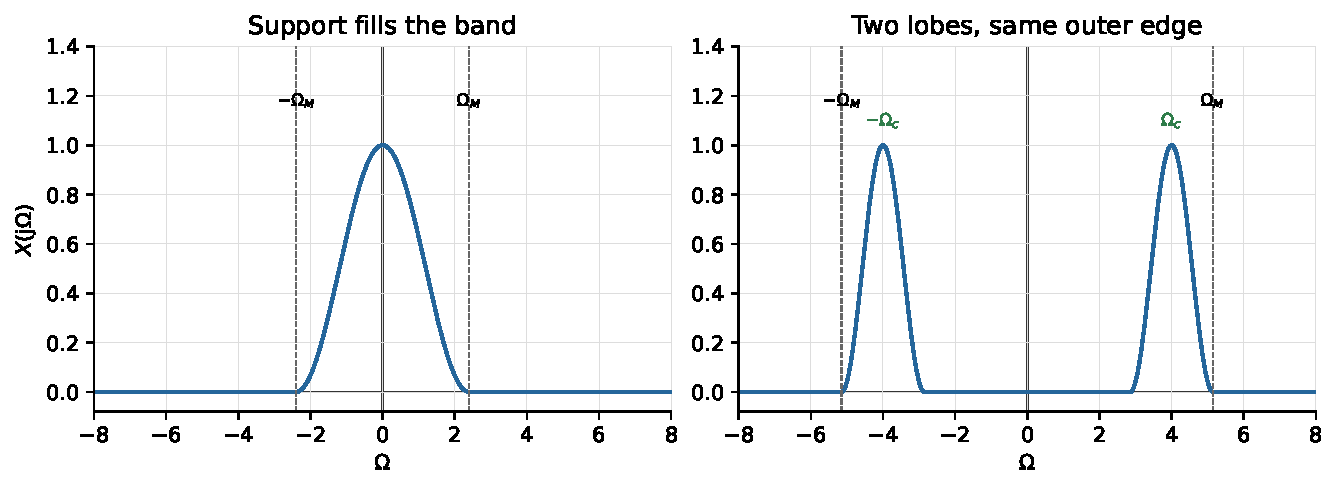
\includegraphics[width=0.88\textwidth]{08-sampling/bandlimited-or.pdf}
    \caption{两种带限支撑。左图占满 $[-\Omega_M,\Omega_M]$；右图只在远离零频的两段上非零，外缘仍是 $\Omega_M$。$\Omega_c$ 只标能量所在的位置，不是采样角频率。}
    \label{fig:sampling-bandlimited-or}
  \end{figure}
  \item 冲激串采样信号由\cref{eq:impulse-sampled-signal}给出，其频谱是原频谱的周期副本：
  \begin{equation}
    X_p(\iu\Omega)
    =\frac1T\sum_{k=-\infty}^{\infty}
      X\bigl(\iu(\Omega-k\Omega_s)\bigr).
    \label{eq:impulse-sampled-spectrum}
  \end{equation}
  每一份副本的高度都乘 $1/T$，相邻副本的间隔是 $\Omega_s$。
  \item 样本序列 $x[n]=x(nT)$ 的离散时间傅里叶变换等于把 $X_p$ 的频率轴按 $T$ 压缩：
  \begin{equation}
    X(\e^{\iu\omega})
    =X_p\Bigl(\iu\frac{\omega}{T}\Bigr)
    =\frac1T\sum_{k=-\infty}^{\infty}
      X\Bigl(\iu\frac{\omega-2\pi k}{T}\Bigr).
    \label{eq:sampling-dtft-replicas}
  \end{equation}
  压缩之后，副本间隔变成 $2\pi$。连续截止落到 $\omega=\pm\Omega_M T$，\cref{fig:sampling-three-relations} 下行用点线标出。\red{离散频率要除以周期}才回到 $\Omega$。
\end{enumerate}

\cref{fig:sampling-three-relations} 的三行分别对应这三种写法。上行为带限连续信号；中行是冲激串及其周期副本，图中副本没有重叠；下行是样本序列和它的 $2\pi$ 周期频谱，阴影是一个主周期，点线是 $\pm\Omega_M T$。

\begin{figure}[H]
  \centering
  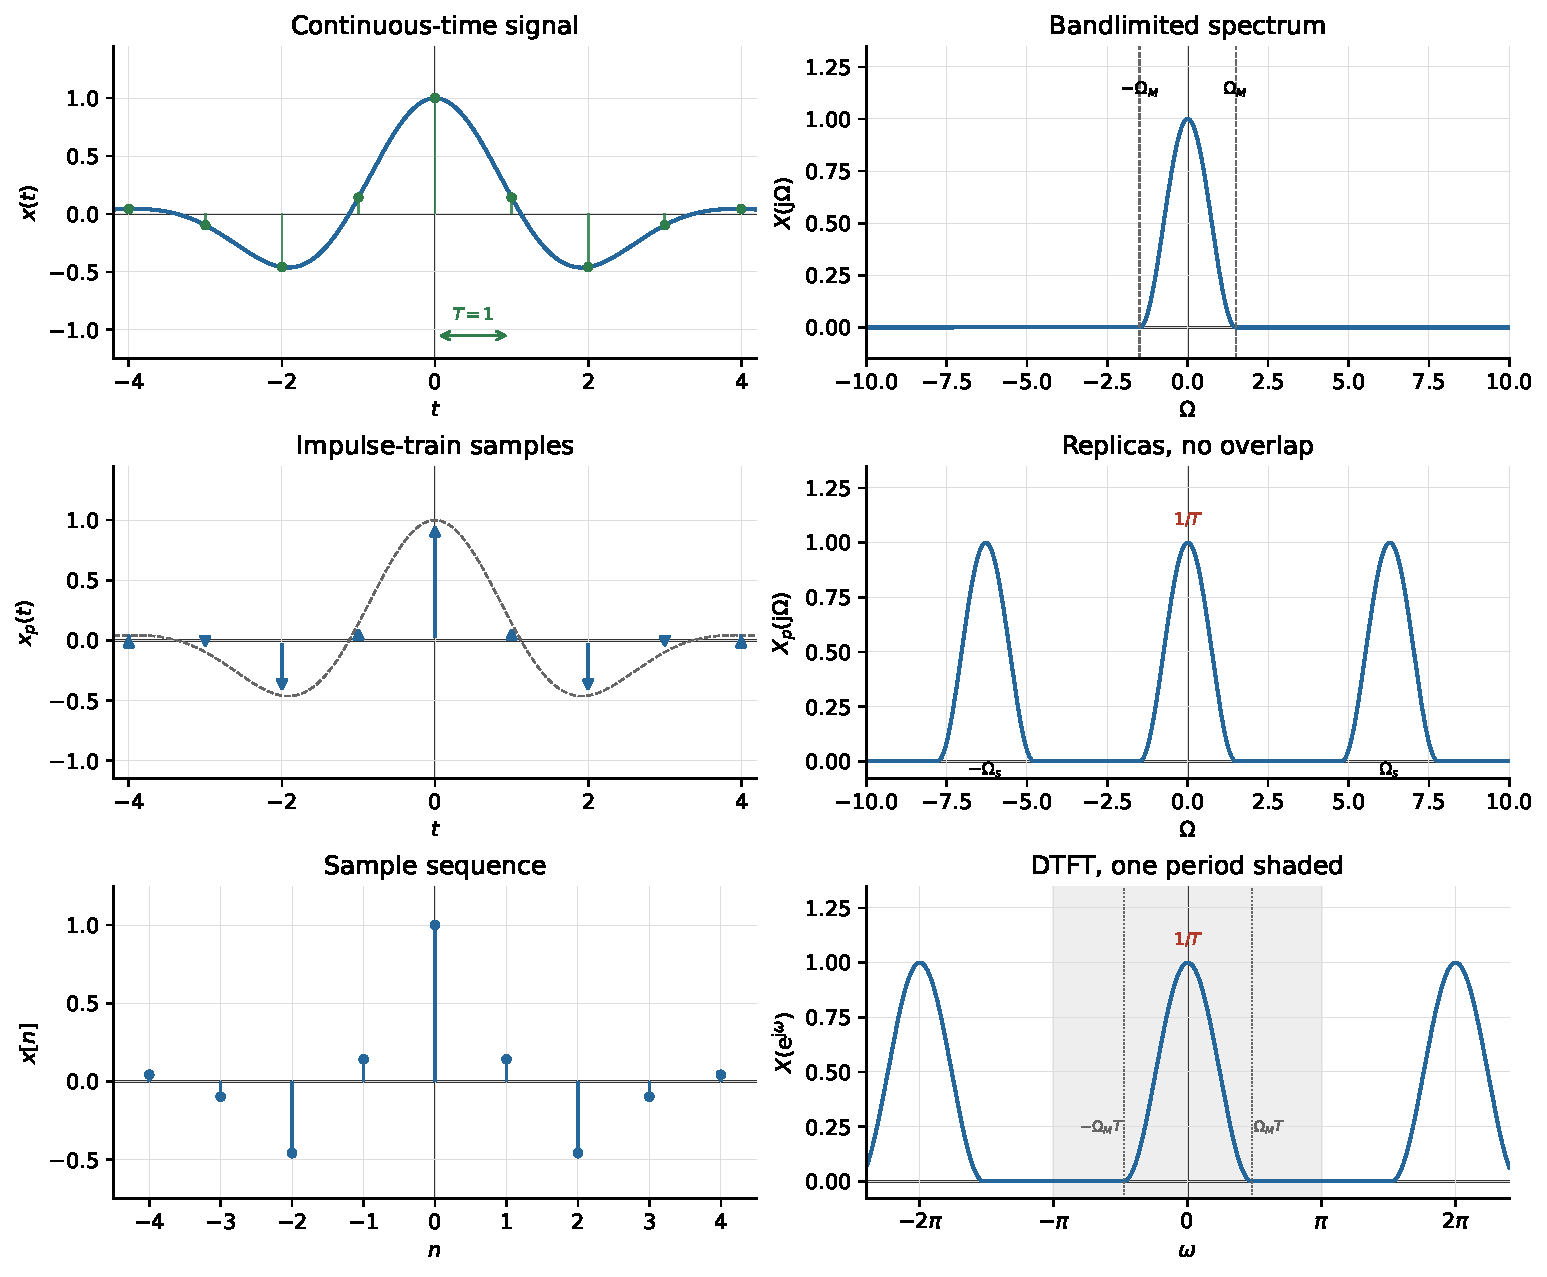
\includegraphics[width=0.96\textwidth]{08-sampling/three-relations.pdf}
  \caption{采样的三组关系，图中取 $T=1$。连续时间频率用 $\Omega$，离散时间频率用 $\omega$。中行冲激权重可正可负，虚线是被采样的 $x(t)$；下行点线是 $\pm\Omega_M T$。$T=1$ 时副本高度与原频谱相同；一般情形仍要乘 $1/T$。}
  \label{fig:sampling-three-relations}
\end{figure}

\subsection{冲激串频谱}
\label{subsec:sampling-impulse-spectrum}

\cref{eq:ctft-impulse-train}把连续时间频率记为 $\omega$、周期记为 $T_0$。这里改用 $\Omega$ 和 $T$，基频 $\Omega_s=2\pi/T$，同一对变换写成
\begin{equation}
  p(t)=\sum_{n=-\infty}^{\infty}\impulse(t-nT)
  \fourierpair
  \Omega_s\sum_{k=-\infty}^{\infty}\impulse(\Omega-k\Omega_s)
  =\frac{2\pi}{T}\sum_{k=-\infty}^{\infty}\impulse(\Omega-k\Omega_s).
  \label{eq:sampling-impulse-train-spectrum}
\end{equation}
系数也可以直接从傅里叶级数读出。在 $(-T/2,T/2)$ 上只有原点的一个冲激，
\[
  a_k=\frac1T\int_{-T/2}^{T/2}\impulse(t)\dd t=\frac1T,
\]
所以
\[
  p(t)=\frac1T\sum_{k=-\infty}^{\infty}\e^{\iu k\Omega_s t}.
\]
再对每一项使用 $\e^{\iu\Omega_0 t}\fourierpair 2\pi\impulse(\Omega-\Omega_0)$，就得到\cref{eq:sampling-impulse-train-spectrum}。各条谱线权重都相同，都是 $2\pi/T$。

$x_p(t)=x(t)p(t)$ 是冲激串调制，频域仍用\cref{eq:ctft-frequency-convolution}。余弦调制只把频谱平移到 $\pm\Omega_0$，\blue{套到冲激串上会漏掉其余副本}。
\[
  X_p(\iu\Omega)
  =\frac1{2\pi}\bigl(X(\iu\,\cdot\,)\conv P(\iu\,\cdot\,)\bigr)(\Omega).
\]
$P$ 是冲激串，与 $\impulse(\Omega-k\Omega_s)$ 卷积只把 $X$ 平移到 $k\Omega_s$。\red{时域相乘走频域卷积}，并且卷积前面有 $1/(2\pi)$：
\begin{align*}
  X_p(\iu\Omega)
  &=\frac1{2\pi}X(\iu\Omega)
    \conv\left[\frac{2\pi}{T}
      \sum_{k=-\infty}^{\infty}\impulse(\Omega-k\Omega_s)\right]\\
  &=\frac1T\sum_{k=-\infty}^{\infty}
    X\bigl(\iu(\Omega-k\Omega_s)\bigr).
\end{align*}
这就是\cref{eq:impulse-sampled-spectrum}。\red{副本高度同乘周期倒数}。平移恒等式 $X(\iu\Omega)\conv\impulse(\Omega-\Omega_0)=X(\iu(\Omega-\Omega_0))$ 在这里逐项使用；漏掉 $1/(2\pi)$ 或把 $2\pi/T$ 再除一次 $T$，副本高度都会错一个周期因子。

\subsection{样本序列的频谱}
\label{subsec:sampling-dtft-link}

第二组关系把连续时间的 $X_p$ 和离散时间的 $X(\e^{\iu\omega})$ 接起来。由\cref{eq:dtft-definition}，
\[
  X(\e^{\iu\omega})
  =\sum_{n=-\infty}^{\infty}x[n]\e^{-\iu\omega n}
  =\sum_{n=-\infty}^{\infty}x(nT)\e^{-\iu\omega n}.
\]
另一方面，
\begin{align*}
  X_p(\iu\Omega)
  &=\int_{-\infty}^{\infty}x_p(t)\e^{-\iu\Omega t}\dd t\\
  &=\int_{-\infty}^{\infty}
    \left[\sum_{n=-\infty}^{\infty}x(nT)\impulse(t-nT)\right]
    \e^{-\iu\Omega t}\dd t\\
  &=\sum_{n=-\infty}^{\infty}x(nT)
    \int_{-\infty}^{\infty}\impulse(t-nT)\e^{-\iu\Omega t}\dd t\\
  &=\sum_{n=-\infty}^{\infty}x(nT)\e^{-\iu\Omega nT}.
\end{align*}
最后一步里，冲激把指数在 $t=nT$ 处取出，剩下的积分是 $1$。\red{该处积分等于一}。令 $\Omega=\omega/T$，
\[
  X_p\Bigl(\iu\frac{\omega}{T}\Bigr)
  =\sum_{n=-\infty}^{\infty}x(nT)\e^{-\iu\omega n}
  =X(\e^{\iu\omega}).
\]
再把\cref{eq:impulse-sampled-spectrum}代进去，并用 $\Omega_s=2\pi/T$，
\begin{align*}
  X(\e^{\iu\omega})
  &=\frac1T\sum_{k=-\infty}^{\infty}
    X\Bigl(\iu\Bigl(\frac{\omega}{T}-k\Omega_s\Bigr)\Bigr)\\
  &=\frac1T\sum_{k=-\infty}^{\infty}
    X\Bigl(\iu\frac{\omega-2\pi k}{T}\Bigr).
\end{align*}
主周期 $[-\pi,\pi]$ 里的 $X(\e^{\iu\omega})$\red{已经包含全部信息}。离散时间频谱本来就以 $2\pi$ 为周期。读连续频率时，用 $\Omega=\omega/T$，不要把 $\omega=\pi$ 直接当成 $\pi\,\mathrm{rad/s}$。

\begin{pitfall}[把两种频率当成同一个数]
  $\omega$ 与 $\Omega$ 相差因子 $T$。$X(\e^{\iu\omega})$ 在 $\omega=\pi$ 处对应的连续频率是 $\Omega=\pi/T=\Omega_s/2$，也就是采样频率的一半。把归一化频率 $\pi$ 当成 $\pi\,\mathrm{rad/s}$，副本位置和低通截止都会差一个 $T$。
\end{pitfall}

\section{采样定理与频谱混叠}
\label{sec:sampling-theorem}

若 $\Omega_s>2\Omega_M$，则 $\Omega_s-\Omega_M>\Omega_M$。$X_p$ 在 $|\Omega|<\Omega_M$ 内只含 $k=0$ 那一份副本，
\[
  X_p(\iu\Omega)=\frac1T X(\iu\Omega),
  \qquad |\Omega|<\Omega_M.
\]
相邻副本从 $\pm\Omega_s$ 开始向两侧展开，最近的边缘在 $\pm(\Omega_s-\Omega_M)$。因此存在截止频率 $\Omega_0$，满足
\begin{equation}
  \Omega_M<\Omega_0<\Omega_s-\Omega_M,
  \label{eq:sampling-cutoff-gap}
\end{equation}
使增益为 $T$ 的理想低通只留下基带副本。低通的频率响应在 $|\Omega|<\Omega_0$ 上为 $T$，在 $|\Omega|>\Omega_0$ 上为 $0$。输出频谱就是 $X(\iu\Omega)$，逆变换回到 $x(t)$。\cref{fig:sampling-reconstruction} 画出副本、低通窗口和恢复后的基带。

\begin{figure}[H]
  \centering
  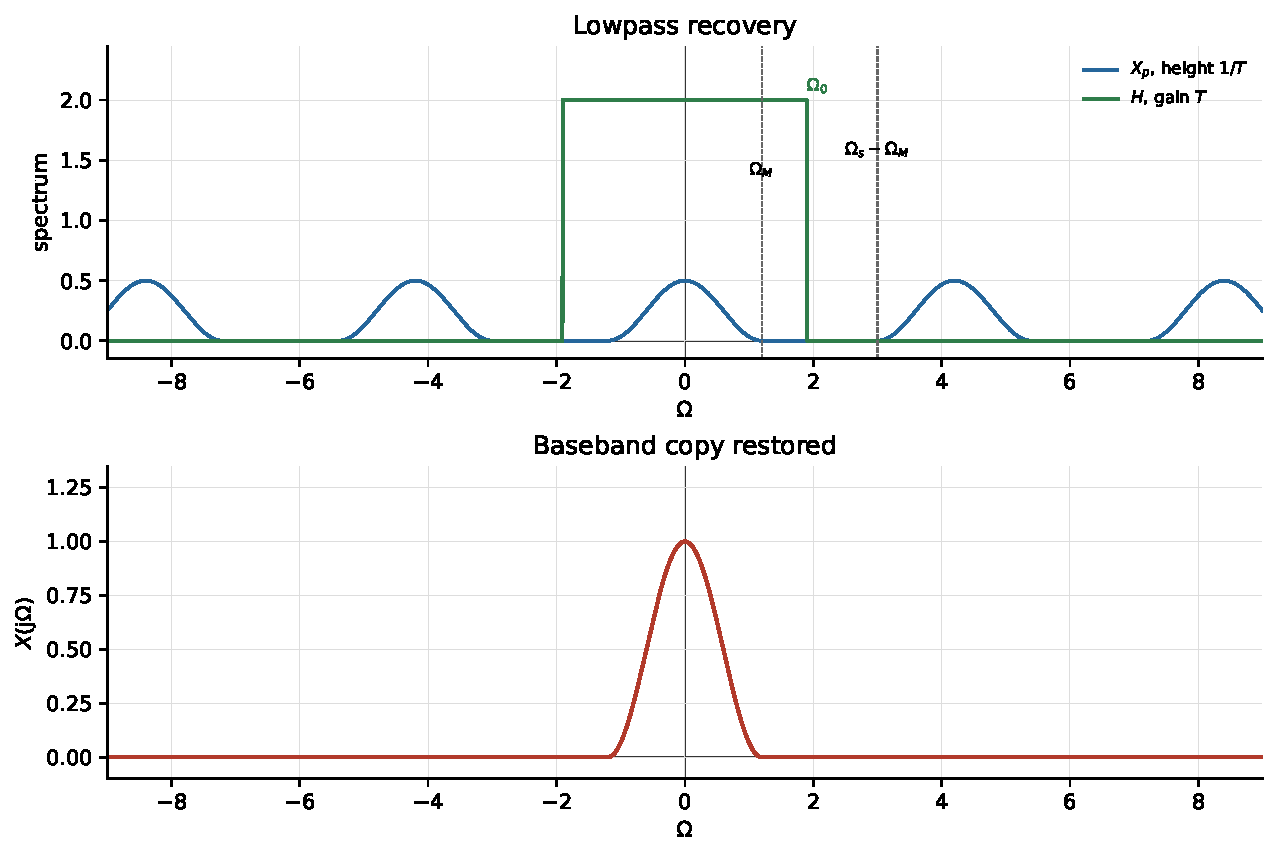
\includegraphics[width=0.86\textwidth]{08-sampling/reconstruction.pdf}
  \caption{由冲激串频谱恢复基带。低通增益为 $T$，截止 $\Omega_0$ 位于 $\Omega_M$ 与 $\Omega_s-\Omega_M$ 之间。下图是低通输出，基带高度已乘回 $T$。}
  \label{fig:sampling-reconstruction}
\end{figure}

\begin{theorem}[采样定理]
  \label{thm:sampling}
  设 $x(t)$ 带限于 $\Omega_M$，即 $|\Omega|>\Omega_M$ 时 $X(\iu\Omega)=0$。若采样角频率满足 $\Omega_s>2\Omega_M$，其中 $\Omega_s=2\pi/T$，则 $x(t)$ 由其样本 $x[n]=x(nT)$，$n\in\Z$，唯一确定。
\end{theorem}

\blue{采样频率必须严格更大}。把恢复过程反过来，就得到唯一性。样本确定 $x_p$，\cref{eq:impulse-sampled-spectrum} 确定全部副本；低通取出基带后，$X$ 被确定，因而 $x$ 被确定。若两个带限信号的样本相同，它们的差在每个 $nT$ 处为零，对应的冲激串为零，基带频谱也为零，这个差就是零信号。

\begin{definition}[奈奎斯特采样频率]
  \label{def:nyquist-rate}
  带限信号最高频率上界 $\Omega_M$ 的两倍 $2\Omega_M$ 称为该信号的\keyterm{奈奎斯特采样频率（Nyquist rate）}。\keyterm{采样定理}要求实际采样角频率严格大于这个值。
\end{definition}

\red{二倍带限上界}。它是采样角频率要超过的那条界，不是采样频率的一半，也不是信号里某条谱线的间隔。换成赫兹时，先把角频率除以 $2\pi$：最高频率 $f_M=\Omega_M/(2\pi)$ 时，每秒样数要大于 $2f_M$。

$\Omega_s$ 比 $2\Omega_M$ 高出越多，\cref{eq:sampling-cutoff-gap} 的空隙越宽，低通的过渡带就可以越宽。\red{间隔越大过渡越宽}。提高采样频率不改变 $x$ 是否带限，只是把副本推开。

等号 $\Omega_s=2\Omega_M$ 不包含在\cref{thm:sampling}里。此时相邻副本在 $\pm\Omega_M$ 相接。若频谱在这两个端点处为零，截止恰好取 $\Omega_s/2$ 仍能把基带分开；若端点处有非零值或冲激，相接处的权重会加在一起，基带不再是原来的一份。\blue{等号时检查端点}。

\subsection{混叠}
\label{subsec:sampling-aliasing}

$\Omega_s<2\Omega_M$ 时，若频谱确实延伸到 $\pm\Omega_M$，相邻副本就会进入对方的支撑，基带里的值变成若干份 $X$ 之和。这种现象称为\keyterm{混叠（aliasing）}。加在一起的副本\red{重叠之后无法拆开}，采样定理的恢复步骤失效。

$\Omega_s>2\Omega_M$ 只保证按这个 $\Omega_M$ 画出的整段支撑不会重叠。\red{它是充分条件}。若实际非零频率低于所写的 $\Omega_M$，或者非零频带之间有空隙、副本正好落进空隙，频谱仍然可以分开。\cref{fig:sampling-aliasing} 的三行依次是：间隔足够时副本分开；支撑填满到 $\Omega_M$ 且间隔不足时重叠区相加；名义上 $\Omega_s<2\Omega_M$，但实际支撑更窄，副本仍然分开。

\begin{figure}[H]
  \centering
  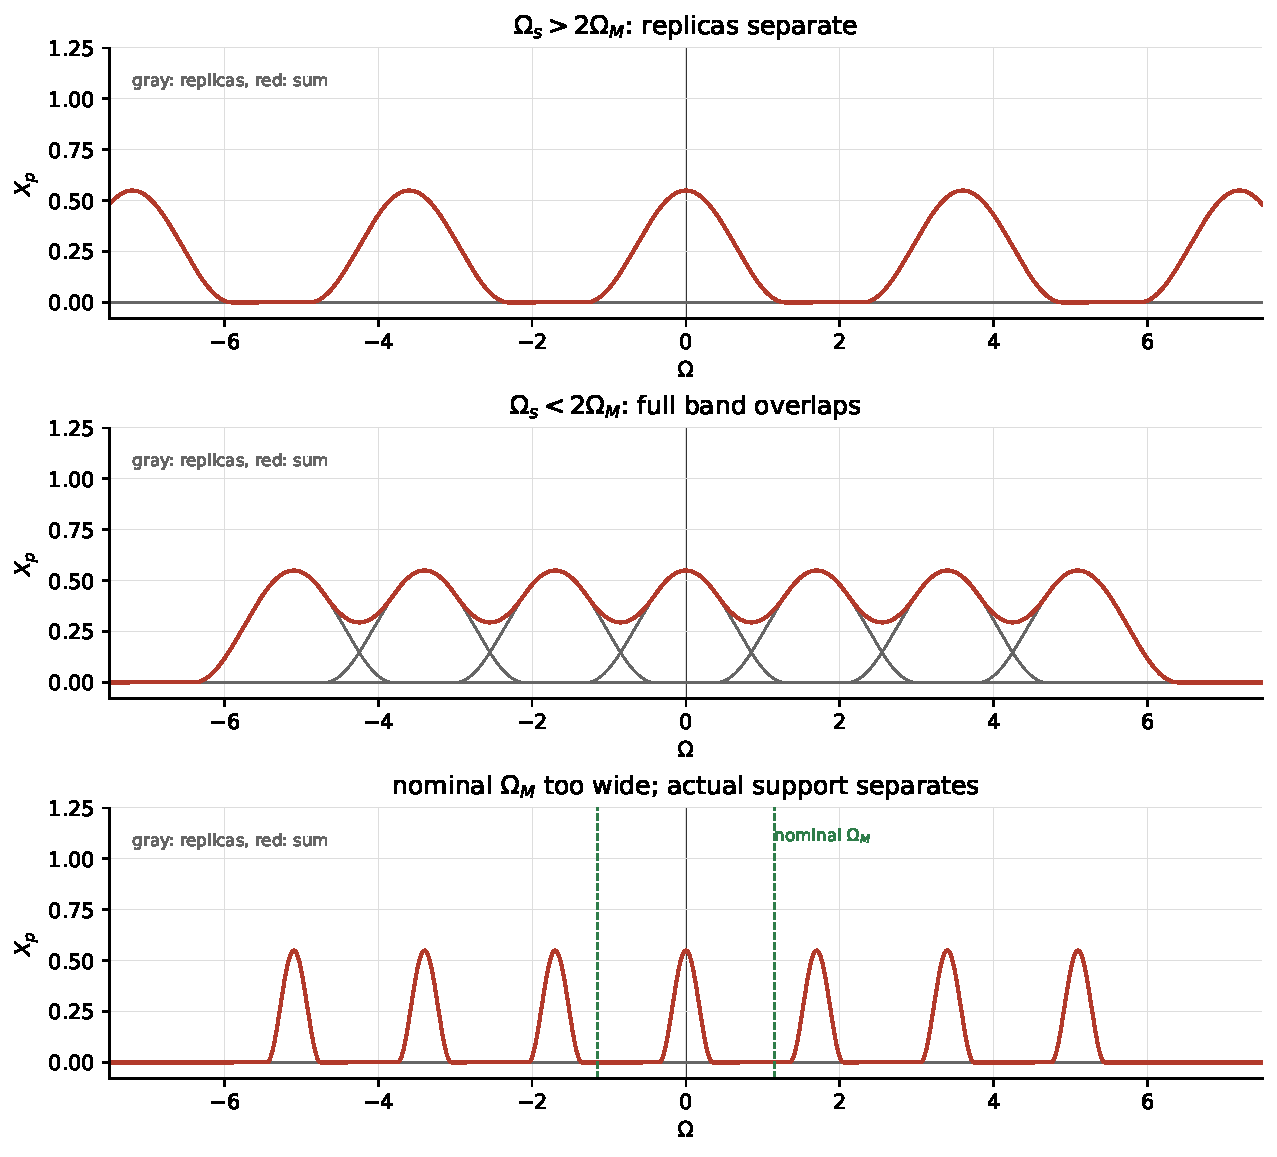
\includegraphics[width=0.84\textwidth]{08-sampling/aliasing.pdf}
  \caption{副本是否重叠取决于实际支撑和 $\Omega_s$。灰线是各份平移，红线是相加后的 $X_p$。第三行的名义截止比实际支撑宽，所以 $\Omega_s<2\Omega_M$ 时仍可能分开。}
  \label{fig:sampling-aliasing}
\end{figure}

\begin{pitfall}[采样偏慢就一定混叠]
  只比较 $\Omega_s$ 和一个偏大的上界，不能推出副本已经相交。$\Omega_M$ 若只是“不超过这个频率”，实际支撑可能更窄，空隙里也可能容纳下一份副本。检查时先画 $X$ 的真实非零区间，再平移 $\Omega_s$，看交集是否为空。\blue{先核对实际支撑}。$\Omega_s>2\Omega_M$ 足够保证不混叠；反过来的不等式不是混叠的判据。
\end{pitfall}

读取 $\Omega_M$ 时按频谱的实际支撑，不按波形看起来“变化有多快”估计。\hl{线谱取最高一条非零谱线}的频率；连续频谱取支撑的外缘。平方之前的截止不能直接当作平方之后的截止，因为时域相乘会在频域把支撑加宽。两个例子分别处理线谱和加宽后的连续谱，见\cref{ex:sampling-nyquist-lines,ex:sampling-sinc-square}。

\section{带限内插}
\label{sec:sampling-interpolation}

采样定理说明样本能够确定 $x(t)$。把这个对应关系写成可计算的和式，还要把 $x_p$ 送进\cref{fig:sampling-reconstruction} 的低通。设低通的冲激响应为 $h$，增益为 $T$，截止为 $\Omega_0$，且 $\Omega_0$ 满足\cref{eq:sampling-cutoff-gap}。由\cref{eq:ctft-sinc-rectangle-pair}，
\[
  h(t)=T\frac{\sin(\Omega_0 t)}{\pi t},
\]
其中 $t=0$ 的值按极限取 $T\Omega_0/\pi$。恢复信号是
\begin{align*}
  x(t)
  &=x_p(t)\conv h(t)\\
  &=\left[\sum_{n=-\infty}^{\infty}x(nT)\impulse(t-nT)\right]
    \conv T\frac{\sin(\Omega_0 t)}{\pi t}.
\end{align*}
与移位冲激卷积等于把 $h$ 平移，所以
\begin{equation}
  x(t)
  =\sum_{n=-\infty}^{\infty}x(nT)\,
    T\frac{\sin\bigl(\Omega_0(t-nT)\bigr)}{\pi(t-nT)}
  =\frac{T}{\pi}\sum_{n=-\infty}^{\infty}
    x[n]\frac{\sin\bigl(\Omega_0(t-nT)\bigr)}{t-nT}.
  \label{eq:sampling-interpolation}
\end{equation}
这是\keyterm{低通内插（bandlimited interpolation）}。\hl{内插先做冲激串}，再与 $\sin(\Omega_0 t)/(\pi t)$ 的 $T$ 倍卷积。两个写法相同：$T/\pi$ 乘 $\sin/(t-nT)$，就是 $T$ 乘 $\sin/[\pi(t-nT)]$。

若取 $\Omega_0=\pi/T=\Omega_s/2$，则 $\Omega_0$ \red{正好处在采样定理允许的区间中点}。此时
\[
  T\frac{\sin\bigl(\pi(t-nT)/T\bigr)}{\pi(t-nT)}
  =\sinc\Bigl(\frac{t-nT}{T}\Bigr),
\]
\cref{eq:sampling-interpolation} 化为
\begin{equation}
  x(t)=\sum_{n=-\infty}^{\infty}
    x(nT)\,\sinc\Bigl(\frac{t-nT}{T}\Bigr).
  \label{eq:sampling-cardinal}
\end{equation}
这里的 $\sinc$ 是\cref{eq:normalized-sinc} 的归一化抽样函数。对整数 $m$，$\sinc(m)=\impulse[m]$：零点处为 $1$，非零整数处为 $0$。因此 $t=mT$ 时，和式只留下 $n=m$ 一项，得到 $x(mT)$。\cref{fig:sampling-interpolation} 把每一项 $\sinc$ 平移和总曲线画在一起，圆点是样本。

\begin{figure}[H]
  \centering
  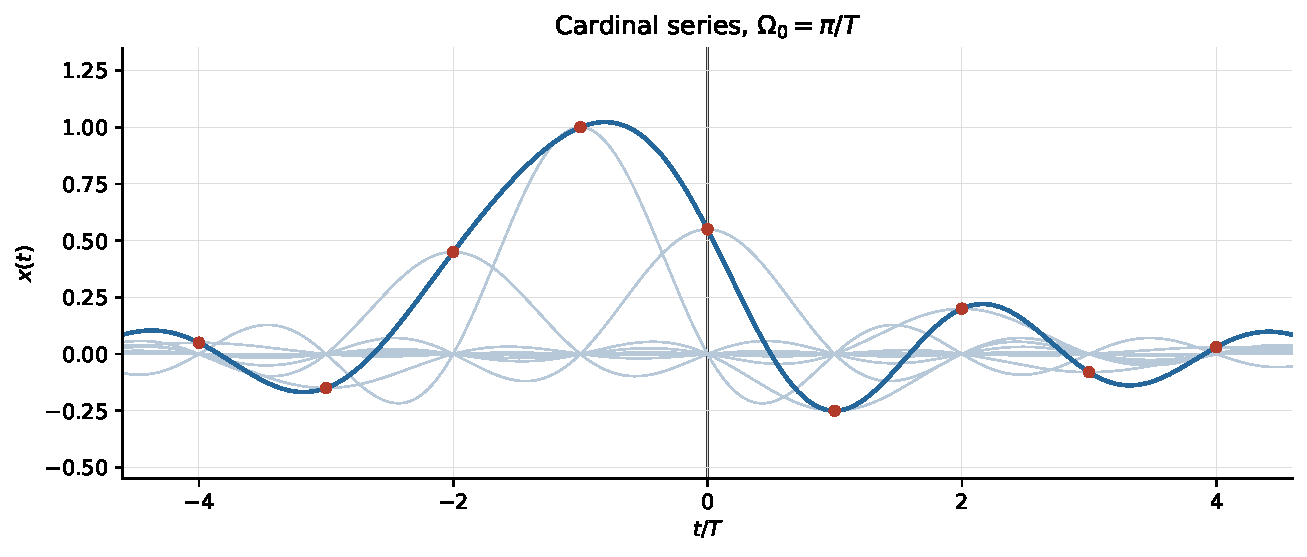
\includegraphics[width=0.88\textwidth]{08-sampling/interpolation.pdf}
  \caption{截止取 $\Omega_s/2$ 时的内插。淡色曲线是各样本乘上移位的 $\sinc$，蓝线是它们的和，红点是 $x(nT)$。}
  \label{fig:sampling-interpolation}
\end{figure}

$\Omega_0\neq\pi/T$ 时，\cref{eq:sampling-interpolation} \blue{在带限且满足采样定理的信号上}仍然等于 $x(t)$，但 $h(kT)$ 一般不再是 $\impulse[k]$。$h(0)=T\Omega_0/\pi$，只有 $\Omega_0=\pi/T$ 时才是 $1$；非零整数 $k$ 处，$\sin(\Omega_0 kT)$ 也不一定为零。任意序列代进这个和式，曲线未必穿过全部样本。带限条件把样本约束住以后，邻项的贡献才正好补成 $x(t)$。\red{半采样频率才穿过样本}。用 $t=nT$ 代入来检查公式时，先看 $\Omega_0$ 是不是 $\pi/T$。

\subsection{带通内插}
\label{subsec:sampling-bandpass-interpolation}

低通留下的是 $k=0$ 副本。若改为留下 $\pm\Omega_s$ 处的两份副本，输出就不再是基带信号。取
\[
  g(t)=T\frac{\sin(\Omega_0 t)}{\pi t}\cos(\Omega_s t).
\]
$\cos(\Omega_s t)$ 把低通频谱各分一半，移到 $\pm\Omega_s$。因此 $g$ 的频率响应在 $|\Omega\pm\Omega_s|<\Omega_0$ 上为 $T/2$，其余为 $0$。$X_p$ 在这两个位置的副本高度是 $1/T$，乘上 $T/2$ 后得到
\[
  \frac12 X\bigl(\iu(\Omega-\Omega_s)\bigr)
  +\frac12 X\bigl(\iu(\Omega+\Omega_s)\bigr),
\]
所得频谱就是 $x(t)\cos(\Omega_s t)$ 的频谱。时域写成
\begin{equation}
  x(t)\cos(\Omega_s t)
  =\frac{T}{\pi}\sum_{n=-\infty}^{\infty}
    x(nT)
    \frac{\sin\bigl(\Omega_0(t-nT)\bigr)}{t-nT}
    \cos\bigl(\Omega_s(t-nT)\bigr).
  \label{eq:sampling-bandpass-interpolation}
\end{equation}
右端与低通内插的差别只是每一项多乘 $\cos[\Omega_s(t-nT)]$。\red{余弦前不再乘二}。\red{带通内插得到调制信号}。\cref{fig:sampling-bandpass} 中，窗口增益是 $T/2$，输出在 $\pm\Omega_s$ 处的高度是原频谱高度的一半。

\begin{figure}[H]
  \centering
  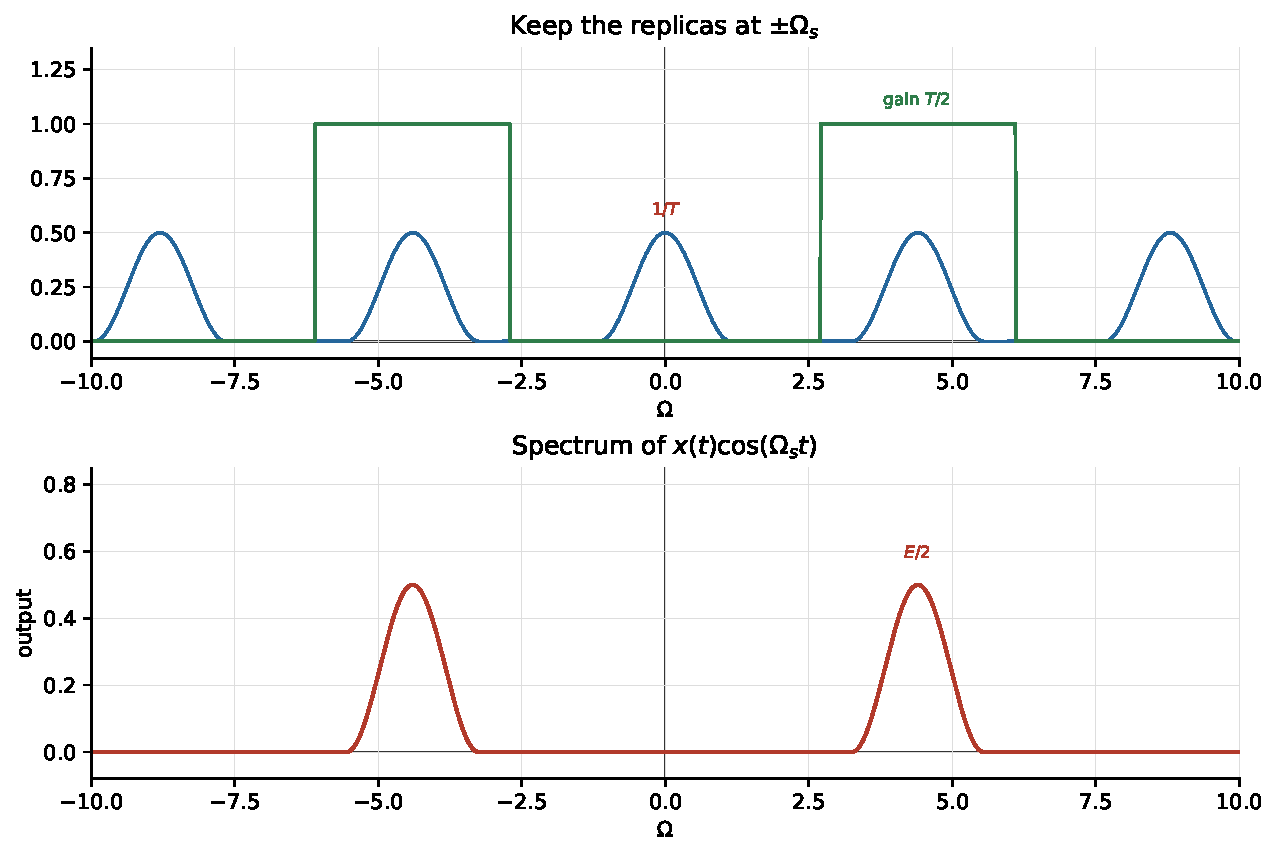
\includegraphics[width=0.86\textwidth]{08-sampling/bandpass-recovery.pdf}
  \caption{保留 $\pm\Omega_s$ 副本。上图绿线是增益为 $T/2$ 的带通窗口；下图是 $x(t)\cos(\Omega_s t)$ 的频谱，高度为原基带的一半。}
  \label{fig:sampling-bandpass}
\end{figure}

\begin{pitfall}[带通公式的左端仍写成原信号]
  \cref{eq:sampling-bandpass-interpolation} 的左端是 $x(t)\cos(\Omega_s t)$。若把左端写成 $x(t)$，等于要求带通窗口同时完成解调。少写 $\cos$ 会回到低通内插；在 $\cos$ 之外再乘 $2$，输出会变成 $2x(t)\cos(\Omega_s t)$。对照图像时\blue{看留下的是零频副本还是} $\pm\Omega_s$ 副本，以及窗口高度是 $T$ 还是 $T/2$。
\end{pitfall}

\section{四组理想滤波器}
\label{sec:sampling-ideal-filters}

内插所用的低通，以及由它平移、取补得到的高通、带通和带阻，可以收成四组增益为 $1$ 的理想滤波器。它们的脉冲响应都是偶函数，相位为零，并且向 $t<0$ 无限延伸，因而都不是因果系统。端点上的有限个函数值不影响逆变换。以下设 $\Omega_0>0$。带通和带阻再设 $\Omega_s>\Omega_0$，使正负两段通带不连在一起。

低通就是\cref{eq:ctft-sinc-rectangle-pair}：
\begin{equation}
  \frac{\sin(\Omega_0 t)}{\pi t}
  \fourierpair
  \mathbf{1}_{|\Omega|<\Omega_0}.
  \label{eq:sampling-ideal-lowpass}
\end{equation}
高通是冲激减去这个低通。$\impulse(t)\fourierpair 1$，所以
\begin{equation}
  \impulse(t)-\frac{\sin(\Omega_0 t)}{\pi t}
  \fourierpair
  \begin{cases}
    0,&|\Omega|<\Omega_0,\\
    1,&|\Omega|>\Omega_0.
  \end{cases}
  \label{eq:sampling-ideal-highpass}
\end{equation}
\red{高通取低通补集}。通带增益是 $1$，不是冲激。

带通把低通调制到 $\pm\Omega_s$。$\cos(\Omega_s t)$ 会把频谱分成两半，要保持通带高度为 $1$，脉冲响应里需要一个 $2$：
\begin{equation}
  \frac{2\sin(\Omega_0 t)}{\pi t}\cos(\Omega_s t)
  \fourierpair
  \mathbf{1}_{|\Omega-\Omega_s|<\Omega_0}
  +\mathbf{1}_{|\Omega+\Omega_s|<\Omega_0}.
  \label{eq:sampling-ideal-bandpass}
\end{equation}
\red{带通要补上二}。带阻再从冲激中减去这一项：
\begin{equation}
  \impulse(t)
  -\frac{2\sin(\Omega_0 t)}{\pi t}\cos(\Omega_s t)
  \fourierpair
  1-\mathbf{1}_{|\Omega-\Omega_s|<\Omega_0}
   -\mathbf{1}_{|\Omega+\Omega_s|<\Omega_0}.
  \label{eq:sampling-ideal-bandstop}
\end{equation}
四组频率响应见\cref{fig:sampling-ideal-filters}。

\begin{figure}[H]
  \centering
  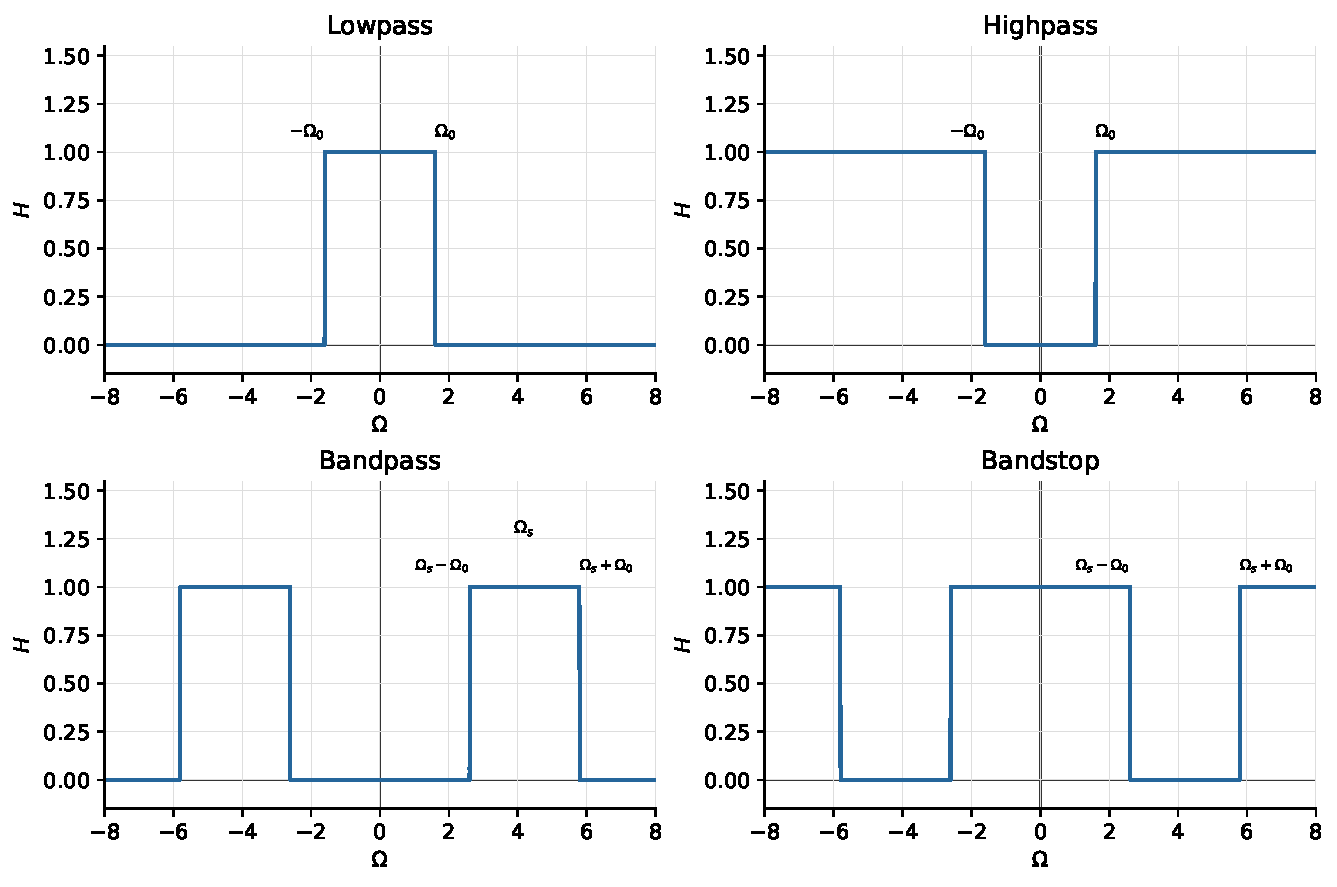
\includegraphics[width=0.92\textwidth]{08-sampling/ideal-filters.pdf}
  \caption{增益为 $1$ 的理想低通、高通、带通和带阻。带通中心在 $\pm\Omega_s$，半宽度为 $\Omega_0$。}
  \label{fig:sampling-ideal-filters}
\end{figure}

这四组的通带高度都是 $1$。\hl{对照表增益为一}。采样恢复不能直接套这张表。基带恢复要把低通增益改成 $T$，脉冲响应相应乘 $T$，用来抵消\cref{eq:impulse-sampled-spectrum}里的 $1/T$。取出 $\pm\Omega_s$ 两份副本时，窗口高度是 $T/2$，脉冲响应写成 $T\sin(\Omega_0 t)\cos(\Omega_s t)/(\pi t)$，余弦前面没有\cref{eq:sampling-ideal-bandpass}里的 $2$。增益为 $1$ 的带通则要把 $\sin(\Omega_0 t)\cos(\Omega_s t)/(\pi t)$ 乘 $2$，正负两段合起来才回到高度 $1$。先核对通带高度，再选系数。

\begin{pitfall}[恢复低通和增益为一的低通用同一个脉冲响应]
  $\sin(\Omega_0 t)/(\pi t)$ 的通带高度是 $1$。采样恢复还要乘 $T$，否则基带只剩下原来的 $1/T$。带通也有两套系数：增益为 $1$ 的带通在 $\cos$ 前乘 $2$；从 $X_p$ 取出 $\pm\Omega_s$ 副本时，窗口高度是 $T/2$，$\cos$ 前不再乘 $2$。两套式子差一个因子时，先核对通带高度。
\end{pitfall}
\section{零阶保持}
\label{sec:sampling-zero-order-hold}

冲激串 $x_p(t)$ 只在采样时刻有冲激。要把每个样本变成持续一段时间的电平，可让它与矩形脉冲卷积。设脉冲宽度 $\tau>0$，
\begin{equation}
  h_0(t)=\stepfun(t)-\stepfun(t-\tau),\qquad
  x_0(t)=x_p(t)\conv h_0(t)
  =\sum_{n=-\infty}^{\infty}x[n]h_0(t-nT).
  \label{eq:sampling-zoh}
\end{equation}
每个冲激在 $nT$ 处产生一个高度为 $x[n]$、宽度为 $\tau$ 的矩形。这里\red{脉冲宽度另用记号}：$T$ 决定样本间隔，$\tau$ 决定电平持续多久。$\tau<T$ 时脉冲之间有空隙；$\tau=T$ 时恰好首尾相接；$\tau>T$ 时\blue{相邻脉冲重叠，电平需要相加}。

\begin{definition}[零阶保持]
  \keyterm{零阶保持（zero-order hold，ZOH）}在 $t=nT$ 读取 $x[n]$，并在 $nT\le t<(n+1)T$ 上保持该值不变。它对应\cref{eq:sampling-zoh} 中的 $\tau=T$：
  \[
    x_0(t)=x[n],\qquad nT\le t<(n+1)T.
  \]
\end{definition}

\red{保持到下一采样时刻}。一个区间内\hl{使用左端的样本值}，样本值变了，电平才跳到下一层。矩形的端点采用上述半开区间约定，不影响频谱。\cref{fig:sampling-hold-shapes} 对照了窄矩形、完整零阶保持和下一节的线性内插。

\begin{figure}[H]
  \centering
  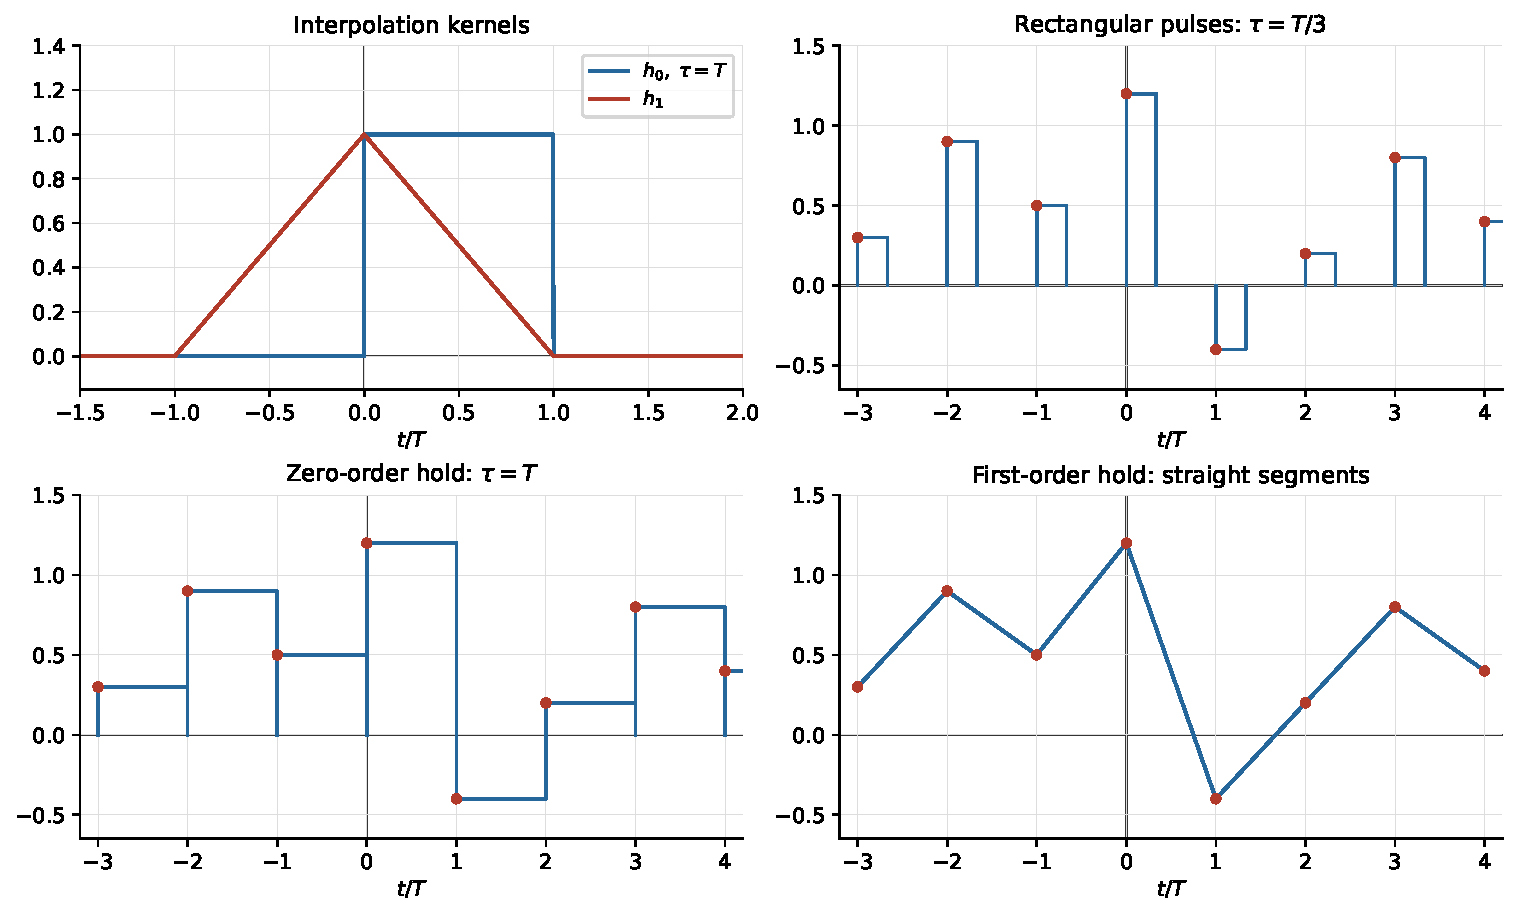
\includegraphics[width=0.94\textwidth]{08-sampling/hold-shapes.pdf}
  \caption{相同样本经不同脉冲内插。左上为矩形、三角形内插核；右上矩形宽度为 $T/3$，脉冲间留有空隙；左下是宽度为 $T$ 的零阶保持；右下用直线连接相邻样本。圆点标出给定样本。}
  \label{fig:sampling-hold-shapes}
\end{figure}

\subsection{保持脉冲的幅度与相位}
\label{subsec:sampling-zoh-spectrum}

直接积分求矩形脉冲的频谱：
\begin{align*}
  H_0(\iu\Omega)
  &=\int_0^\tau \e^{-\iu\Omega t}\dd t
   =\frac{1-\e^{-\iu\Omega\tau}}{\iu\Omega}\\
  &=\e^{-\iu\Omega\tau/2}
    \frac{2\sin(\Omega\tau/2)}{\Omega}.
\end{align*}
用第二章的 $\Sa(v)=\sin v/v$ 记号，
\begin{equation}
  H_0(\iu\Omega)
  =\tau\Sa\Bigl(\frac{\Omega\tau}{2}\Bigr)
       \e^{-\iu\Omega\tau/2},
  \qquad
  X_0(\iu\Omega)=X_p(\iu\Omega)H_0(\iu\Omega).
  \label{eq:sampling-zoh-spectrum}
\end{equation}
$\Omega=0$ 处按极限取 $H_0(0)=\tau$。零点在 $\Omega=2k\pi/\tau$，$k\ne0$。幅度为 $\tau|\Sa(\Omega\tau/2)|$；在第一对零点之间，$\Sa$ 为正，相位是 $-\Omega\tau/2$。\red{矩形中心带来延时}，对应延时量 $\tau/2$。过了零点后，$\Sa$ 的符号还会使相位增加或减少 $\pi$，不能把整个实轴上的相位都画成同一条直线；\blue{零点处相位未定义}。

取 $\tau=T$。在没有混叠的基带内，$X_p=X/T$，于是
\[
  X_0(\iu\Omega)
  =X(\iu\Omega)\Sa\Bigl(\frac{\Omega T}{2}\Bigr)
       \e^{-\iu\Omega T/2}.
\]
零频增益为 $1$，其余频率按 $\Sa$ 衰减，还附带 $T/2$ 的延时。\red{保持后仍有频谱副本}，矩形频谱只压低副本，并没有把它们完全去掉。阶梯形 $x_0(t)$ 因而通常只是 $x(t)$ 的近似。

\subsection{零阶保持后的精确恢复}
\label{subsec:sampling-zoh-recovery}

设输入满足采样定理，恢复低通截止 $\Omega_0$ 满足\cref{eq:sampling-cutoff-gap}。冲激串直接恢复需要通带增益 $T$；在 $h_0$ 后增加滤波器 $C_0$，就要求通带内 $H_0C_0=T$。因此
\begin{equation}
  C_0(\iu\Omega)=
  \begin{cases}
    \dfrac{T}{\tau\Sa(\Omega\tau/2)}
       \e^{\iu\Omega\tau/2},&|\Omega|<\Omega_0,\\[0.7em]
    0,&|\Omega|>\Omega_0.
  \end{cases}
  \label{eq:sampling-zoh-compensation}
\end{equation}
通带内还需 $H_0$ 无零点。例如 $0<\tau\le T$、$\Omega_0=\pi/T$ 就满足此条件。此时 $X_0C_0=X$，恢复时同时\red{补偿幅度与延时}。宽度取 $\tau=T$ 时，通带内
\[
  |C_0(\iu\Omega)|=\frac1{\Sa(\Omega T/2)},\qquad
  \arg C_0(\iu\Omega)=\frac{\Omega T}{2}.
\]
高频衰减更大，补偿幅度也更大；正的相位斜率用来抵消保持脉冲的延时。\blue{通带不能包含保持零点}，\red{否则所需补偿增益无界}。这是理想恢复模型，精确的频带截断和时间超前不能直接由一个因果滤波器实现。\cref{fig:sampling-hold-spectra} 将保持与补偿的幅相放在一起。

\begin{pitfall}[保持后只接增益为一的理想低通]
  增益为一的低通能去掉频谱副本，但保留下来的基带仍乘着 $\Sa(\Omega T/2)\e^{-\iu\Omega T/2}$。要精确恢复，须按\cref{eq:sampling-zoh-compensation} 补回幅度与相位。脉冲宽度不等于 $T$ 时，零频补偿增益还要改为 $T/\tau$。
\end{pitfall}

\section{一阶保持与线性内插}
\label{sec:sampling-first-order-hold}

零阶保持每段是常数。若希望曲线连续，可用直线连接相邻样本，这称为线性内插（linear interpolation），这里也称\keyterm{一阶保持（first-order hold，FOH）}。相应的内插核是顶点高度为 $1$ 的对称三角脉冲：
\begin{equation}
  h_1(t)=
  \begin{cases}
    1-\dfrac{|t|}{T},&|t|<T,\\[0.4em]
    0,&|t|\ge T,
  \end{cases}
  \qquad
  x_1(t)=x_p(t)\conv h_1(t)
        =\sum_n x[n]h_1(t-nT).
  \label{eq:sampling-foh}
\end{equation}
在 $nT\le t\le(n+1)T$ 内，只有以 $nT$ 和 $(n+1)T$ 为中心的两份三角脉冲有贡献。令 $\alpha=(t-nT)/T$，得到
\begin{equation}
  x_1(t)=(1-\alpha)x[n]+\alpha x[n+1],
  \qquad 0\le\alpha\le1.
  \label{eq:sampling-linear-interpolation}
\end{equation}
两项权重之和为 $1$；从区间左端到右端，前一个权重从 $1$ 减到 $0$，后一个从 $0$ 增到 $1$。\red{相邻样本直线相连}，见\cref{fig:sampling-hold-shapes} 右下图。曲线连续，但样本处的斜率一般会改变。

求三角脉冲的频谱时，令 $r(t)=1$（$|t|<T/2$），其余为零。两个矩形卷积的重叠长度是 $T-|t|$，所以 $h_1=(r\conv r)/T$。由矩形变换对，
\begin{equation}
  H_1(\iu\Omega)
  =\frac1T\left[T\Sa\Bigl(\frac{\Omega T}{2}\Bigr)\right]^2
  =T\Sa^2\Bigl(\frac{\Omega T}{2}\Bigr),
  \qquad X_1=X_pH_1.
  \label{eq:sampling-foh-spectrum}
\end{equation}
\red{三角脉冲对应平方}。$H_1$ 实且非负，非零处的相位为 $0$，零点处相位未定义；第一对零点仍在 $\pm2\pi/T$。第一对零点之间，$\Sa^2$ 比 $\Sa$ 更小，一阶保持的基带幅度也有衰减。

\blue{输入满足采样定理时}，$X_1=X\Sa^2(\Omega T/2)$ 在基带成立。精确恢复需要
\begin{equation}
  C_1(\iu\Omega)=
  \begin{cases}
    \dfrac1{\Sa^2(\Omega T/2)},&|\Omega|<\Omega_0,\\[0.7em]
    0,&|\Omega|>\Omega_0,
  \end{cases}
  \label{eq:sampling-foh-compensation}
\end{equation}
其中 $\Omega_0$ 满足\cref{eq:sampling-cutoff-gap} 且 $\Omega_0<2\pi/T$；取 $\pi/T$ 即可。通带内 $C_1H_1=T$，所以 $X_1C_1=X$。\red{直线内插仍需补偿}，穿过样本和精确恢复整条曲线是两个要求。

\begin{figure}[H]
  \centering
  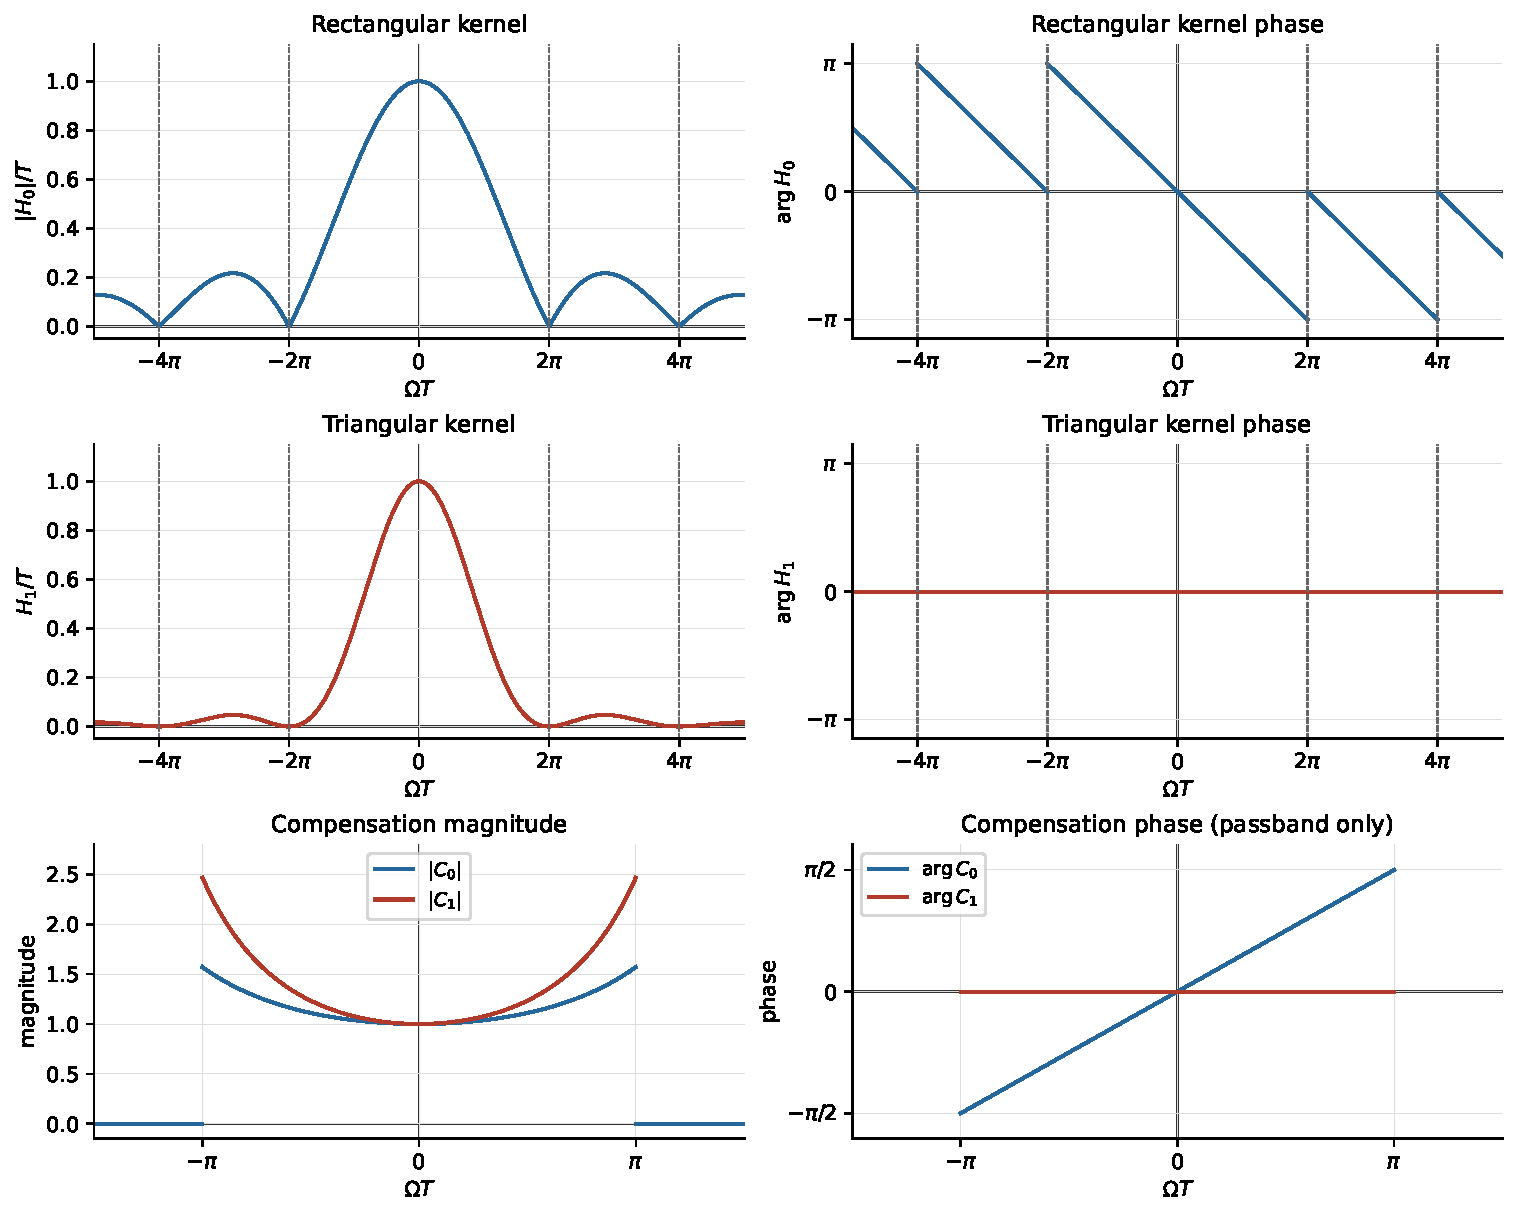
\includegraphics[width=0.94\textwidth]{08-sampling/hold-spectra.pdf}
  \caption{保持与恢复的幅相，横坐标为 $\Omega T$，零阶保持取 $\tau=T$。上两行分别是矩形与三角脉冲的频谱；虚线标零点，零点处不画相位值。下行是截止为 $\pi/T$ 时的补偿：蓝线补零阶保持，红线补一阶保持；通带之外幅度为零，相位未定义。}
  \label{fig:sampling-hold-spectra}
\end{figure}

\begin{pitfall}[线性内插可以立即用当前样本输出]
  \cref{eq:sampling-linear-interpolation} 用到了 $x[n+1]$。在 $nT<t<(n+1)T$ 时，下一个样本尚未到达，所以此处的对称三角核是非因果的。若允许延时 $T$，可改用 $h_1(t-T)$：在当前区间内画出前一个区间的连线，输出为 $x_1(t-T)$。延时版本的频谱还要乘 $\e^{-\iu\Omega T}$。
\end{pitfall}

\section{连续时间 LTI 系统的离散实现}
\label{sec:sampling-discrete-implementation}

设连续时间系统的频率响应为 $H(\iu\Omega)$，希望得到
\[
  y(t)=x(t)\conv h(t),\qquad
  Y(\iu\Omega)=X(\iu\Omega)H(\iu\Omega).
\]
一条实现路线是\hl{先采样，再作离散卷积}，最后恢复连续输出：
\[
  x(t)\longrightarrow\boxed{\text{采样}}
  \longrightarrow x[n]\longrightarrow\boxed{h_d[n]}
  \longrightarrow y[n]\longrightarrow\boxed{\text{恢复}}
  \longrightarrow y(t).
\]
这里 $x[n]=x(nT)$，$y[n]=y(nT)$，离散系统的频率响应记为 $H_d(\e^{\iu\omega})$。\cref{fig:sampling-discrete-flow} 将恢复部分展开成“序列变冲激串、零阶保持、补偿滤波”。

\begin{figure}[H]
  \centering
  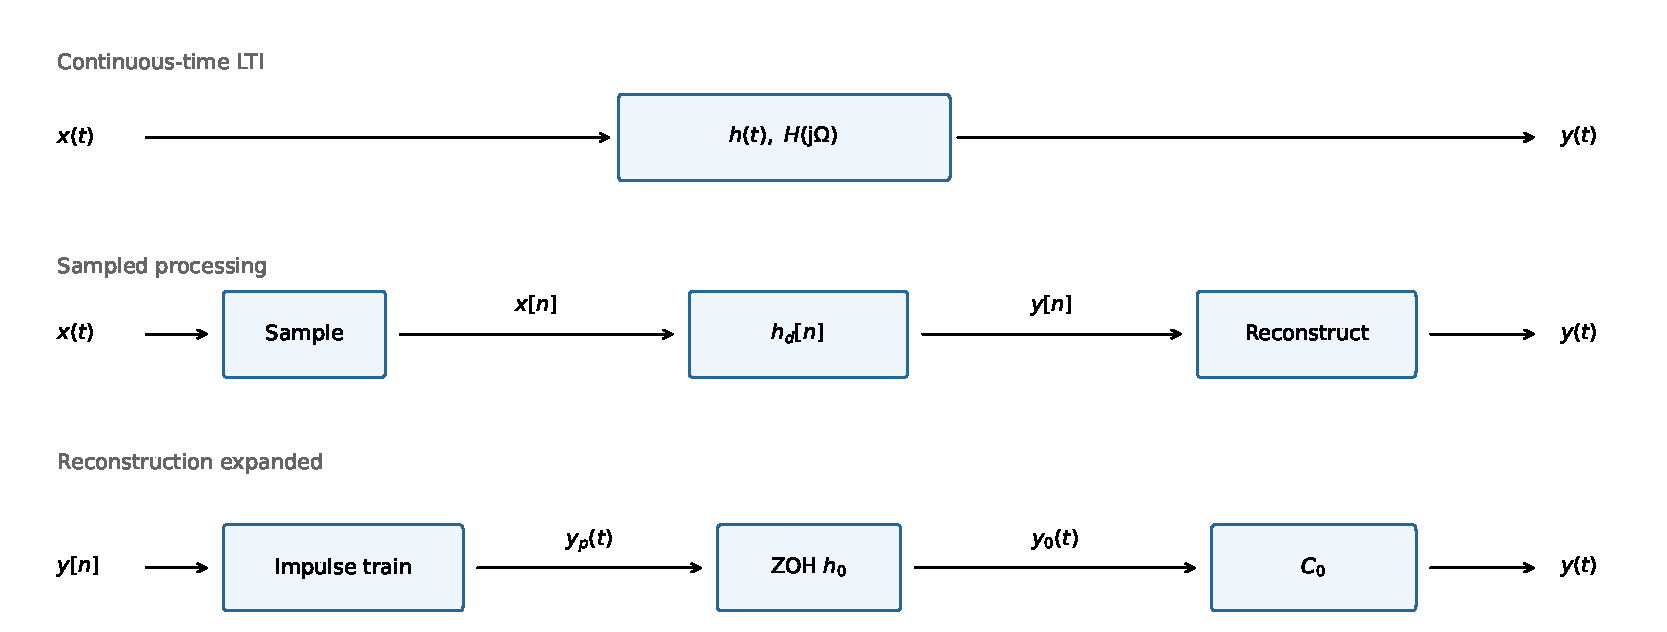
\includegraphics[width=0.96\textwidth]{08-sampling/discrete-system-flow.pdf}
  \caption{连续系统与离散处理路线。下方的 $y[n]$ 先变成冲激串 $y_p(t)$，经过矩形保持得到 $y_0(t)$，再由 $C_0$ 恢复。保持和补偿的总频率响应等于增益为 $T$ 的恢复低通。}
  \label{fig:sampling-discrete-flow}
\end{figure}

\subsection{频率响应应怎样对应}
\label{subsec:sampling-discrete-response}

假定 $x$ 带限于 $\Omega_M<\pi/T$。在主周期 $-\pi<\omega<\pi$ 内，采样后的频谱由\cref{eq:sampling-dtft-replicas} 化为
\[
  X(\e^{\iu\omega})=\frac1T X\Bigl(\iu\frac{\omega}{T}\Bigr).
\]
离散滤波得到 $Y(\e^{\iu\omega})=X(\e^{\iu\omega})H_d(\e^{\iu\omega})$。把 $y[n]$ 变回间隔为 $T$ 的冲激串，其频谱为 $Y_p(\iu\Omega)=Y(\e^{\iu\Omega T})$。恢复低通的通带增益为 $T$，故在 $|\Omega|<\pi/T$ 内
\begin{align*}
  Y_{\mathrm{out}}(\iu\Omega)
  &=T Y(\e^{\iu\Omega T})\\
  &=T\left[\frac1T X(\iu\Omega)\right]
    H_d(\e^{\iu\Omega T})\\
  &=X(\iu\Omega)H_d(\e^{\iu\Omega T}).
\end{align*}
因此，应在一个主周期内选取
\begin{equation}
  H_d(\e^{\iu\omega})=H\Bigl(\iu\frac{\omega}{T}\Bigr),
  \qquad -\pi<\omega<\pi,
  \label{eq:sampling-system-frequency-link}
\end{equation}
再作 $2\pi$ 周期延拓。\red{系统增益不再除以周期}：输入采样时的 $1/T$ 已被输出恢复的 $T$ 抵消。连续频率 $\Omega$ 对应离散频率 $\omega=\Omega T$，一个离散周期只对应连续区间 $[-\pi/T,\pi/T]$。

实现某一带限输入时，只需要在该输入的频谱支撑上满足这条响应关系。在主周期其他位置如何选取 $H_d$，不会改变这个输入的输出。\red{对应只看输入占用频带}。\cref{fig:sampling-system-spectra} 按三列画出输入、系统响应和输出，连续与离散的频谱高度并不全都相同。

\begin{figure}[H]
  \centering
  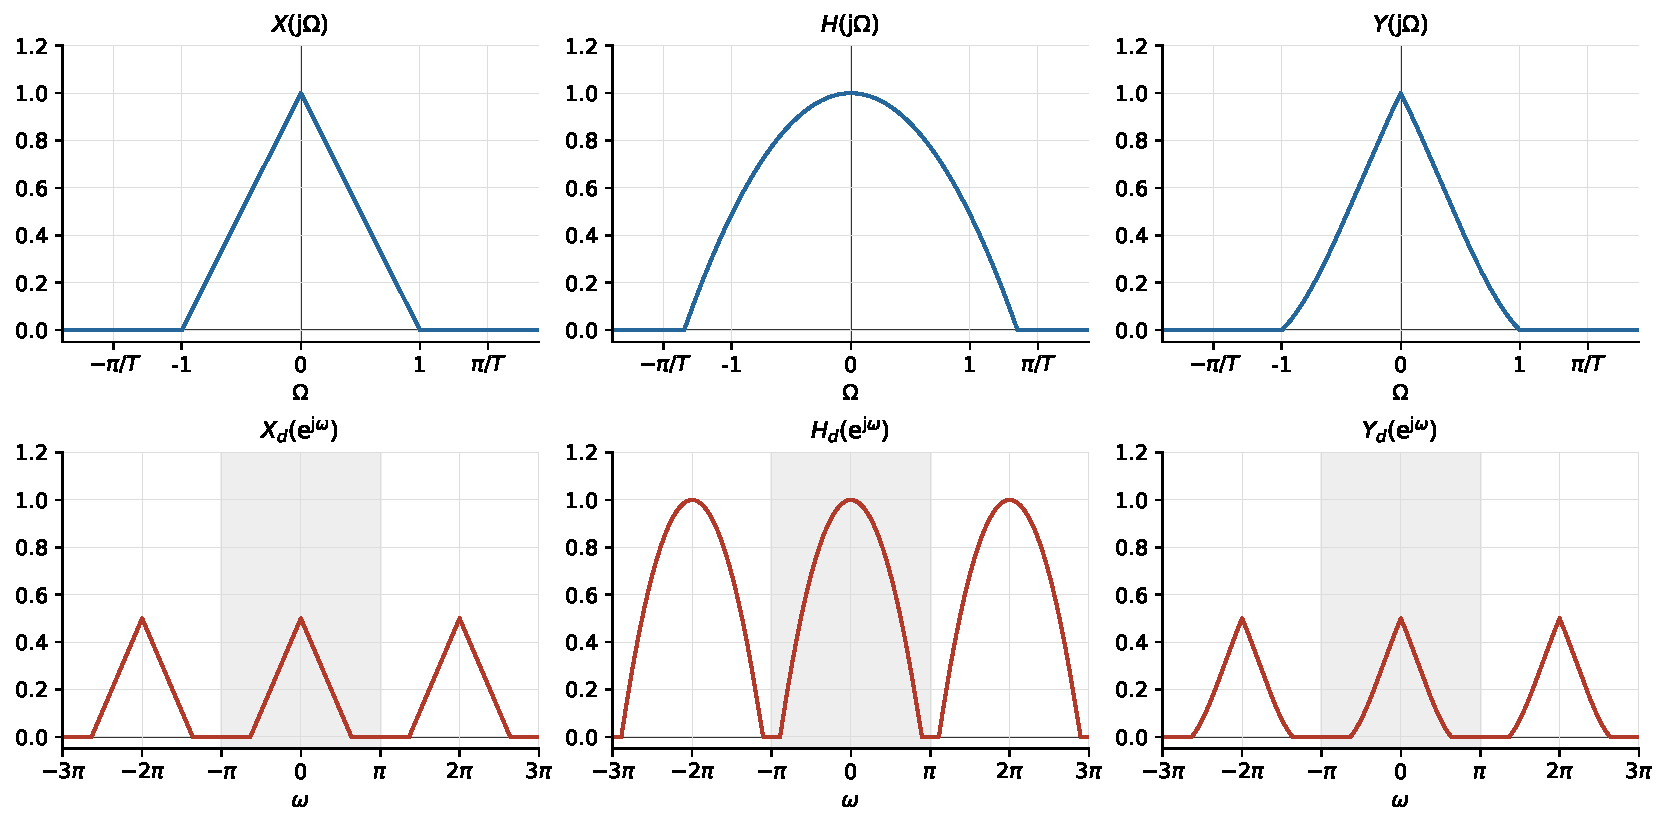
\includegraphics[width=0.96\textwidth]{08-sampling/discrete-system-spectra.pdf}
  \caption{连续与离散的系统关系，取 $T=2$。上行满足 $Y=XH$；下行满足 $Y_d=X_dH_d$。输入、输出的采样副本高度各乘 $1/T$，系统响应 $H_d$ 的高度与连续响应 $H$ 相同。灰色区为离散频谱的一个主周期。}
  \label{fig:sampling-system-spectra}
\end{figure}

采样器本身不满足连续时间的时不变性：一个窄脉冲平移后可能落到采样点之间，从而完全漏采。上面的等效 LTI 关系依赖输入带限，\blue{带限条件保证系统等效}。对任意输入，不能把整条采样处理路线直接当作同一个连续 LTI 系统。

\subsection{离散脉冲响应为什么多一个周期}
\label{subsec:sampling-impulse-response-link}

若 $H(\iu\Omega)$ 也带限于 $\pi/T$ 内，$h(t)$ 的采样频谱满足
\[
  h(nT)\fourierpair
  \frac1T\sum_k H\Bigl(\iu\frac{\omega-2\pi k}{T}\Bigr).
\]
主周期内只有 $k=0$ 副本。乘上 $T$，恰好得到\cref{eq:sampling-system-frequency-link} 要求的响应：
\begin{equation}
  h_d[n]=T h(nT).
  \label{eq:sampling-discrete-impulse-response}
\end{equation}
\red{脉冲响应要乘采样周期}。连续卷积积分中的时间宽度，在离散卷积和里由这个 $T$ 承担。

也可沿时域核对。设 $h$ 带限于 $\Omega_h<\pi/T$，$x$ 带限于 $\Omega_M<\pi/T$，内插级数与卷积允许换序。将\cref{eq:sampling-cardinal} 代入连续卷积：
\[
  y(t)=\sum_k x[k]\left[
    \sinc\Bigl(\frac{t-kT}{T}\Bigr)\conv h(t)\right].
\]
括号内的 $\sinc$ 频谱在 $|\Omega|<\pi/T$ 上为 $T$，与 $H$ 相乘后就是 $T H(\iu\Omega)\e^{-\iu\Omega kT}$，所以括号等于 $T h(t-kT)$。在 $t=nT$ 取样，
\[
  y[n]=\sum_k x[k]\,T h((n-k)T)
      =\sum_k x[k]h_d[n-k].
\]
这里先用带限内插，再作精确卷积，不能把它理解成对任意函数都成立的数值积分近似。

\begin{pitfall}[直接采样任意脉冲响应]
  任意 $h$ 的采样会使 $H$ 的副本相加，$T h(nT)$ 一般不满足\cref{eq:sampling-system-frequency-link}。\blue{先检查系统是否带限}。若 $H$ 不带限，可先截取主频带：
  \[
    H_b(\iu\Omega)=
    \begin{cases}
      H(\iu\Omega),&|\Omega|<\pi/T,\\
      0,&|\Omega|>\pi/T.
    \end{cases}
  \]
  令 $h_b$ 为其逆变换，再取 $h_d[n]=T h_b(nT)$。在满足采样定理的输入上，截掉输入本来没有的频率\red{不会改变连续输出}。
\end{pitfall}

\section{连续信号与样本序列的能量}
\label{sec:sampling-energy}

满足采样定理时，样本能确定整条波形。连续能量对时间积分，离散能量对样值求和，\red{两者还相差一个时间因子}。设
\[
  E_c=\int_{-\infty}^{\infty}|x(t)|^2\dd t<\infty,
  \qquad
  E_d=\sum_{n=-\infty}^{\infty}|x[n]|^2.
\]
若 $x$ 带限于 $\Omega_M<\pi/T$，则主周期内 $X(\e^{\iu\omega})=X(\iu\omega/T)/T$。使用第六、七章的帕塞瓦尔关系，
\begin{align*}
  E_d
  &=\frac1{2\pi}\int_{-\pi}^{\pi}
       |X(\e^{\iu\omega})|^2\dd\omega\\
  &=\frac1{2\pi T^2}\int_{-\pi}^{\pi}
       \left|X\Bigl(\iu\frac{\omega}{T}\Bigr)\right|^2\dd\omega\\
  &\underset{\Omega=\omega/T}{=}
       \frac1{2\pi T}\int_{-\pi/T}^{\pi/T}|X(\iu\Omega)|^2\dd\Omega\\
  &=\frac1T\left[
       \frac1{2\pi}\int_{-\infty}^{\infty}|X(\iu\Omega)|^2\dd\Omega
     \right]
   =\frac{E_c}{T}.
\end{align*}
第三行代换时 $\dd\omega=T\dd\Omega$；第四行把积分扩至全实轴，是因为区间外频谱为零。于是
\begin{equation}
  \int_{-\infty}^{\infty}|x(t)|^2\dd t
  =T\sum_{n=-\infty}^{\infty}|x(nT)|^2.
  \label{eq:sampling-energy}
\end{equation}
\blue{能量求和还要乘周期}。采样越密，参与求和的样值越多；乘上每一格的时间宽度 $T$，才得到连续能量。\red{这是在上述条件下的精确等式}。

例如 $x(t)=\sin(\pi t)/(\pi t)=\sinc(t)$，$X(\iu\Omega)$ 是高度 $1$、宽度 $2\pi$ 的矩形，故 $E_c=1$。取 $T=1/2$ 和 $T=1/4$，采样频率均严格超过 $2\pi$，样本序列能量分别为 $2$ 和 $4$，乘上对应 $T$ 后都为 $1$。\cref{fig:sampling-energy} 对照两组样本及能量。

\begin{figure}[H]
  \centering
  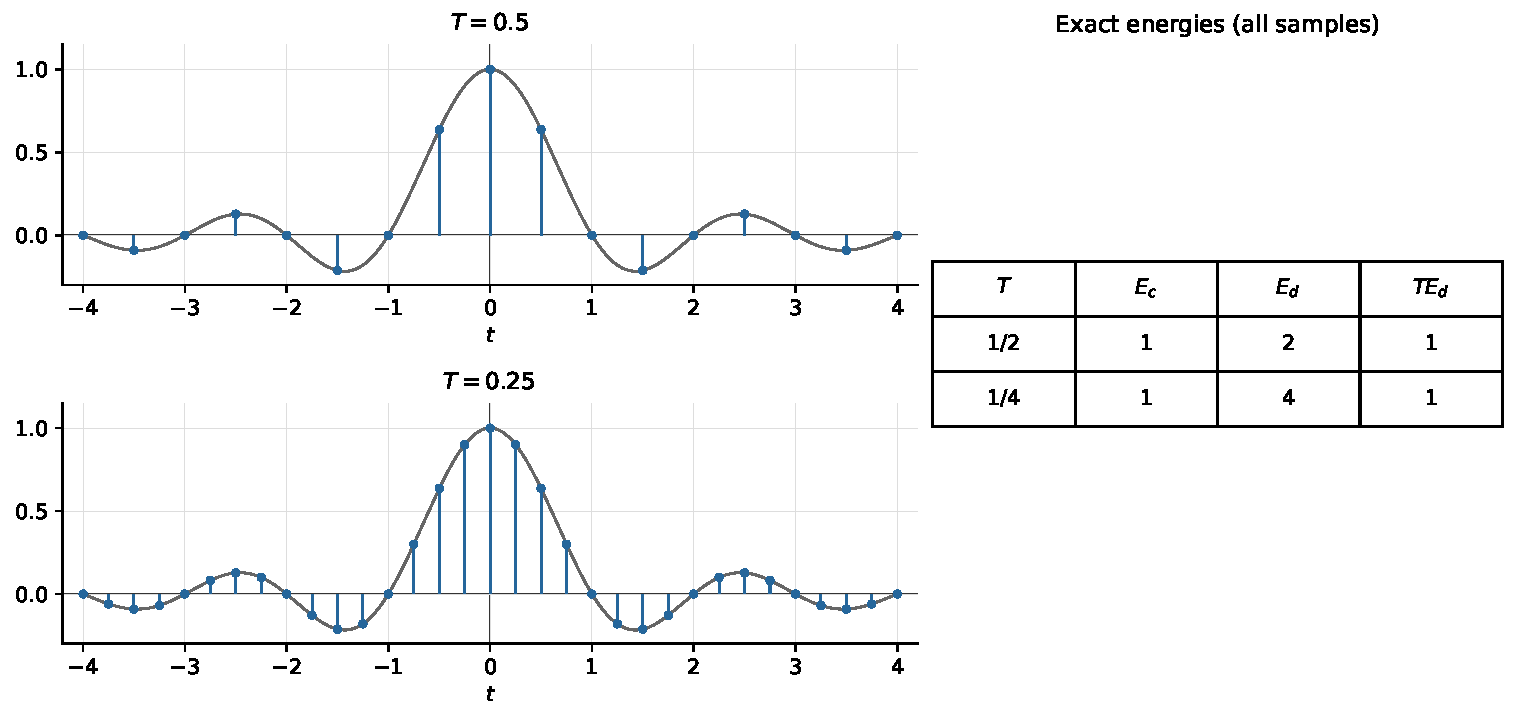
\includegraphics[width=0.9\textwidth]{08-sampling/sample-energy.pdf}
  \caption{$\sinc(t)$ 的两组样本。左侧只画有限时间窗口，右侧数值按全序列的精确公式给出。$T$ 减半，离散能量加倍；$T E_d$ 始终等于连续能量 $1$。}
  \label{fig:sampling-energy}
\end{figure}

若信号不带限，\cref{eq:sampling-energy} 一般失效。取
\[
  q(t)=
  \begin{cases}
    1,&T/4<t<3T/4,\\
    0,&\text{其余},
  \end{cases}
\]
全部 $q(nT)=0$，样本能量为 $0$，连续能量却为 $T/2$。\blue{非带限信号不能照套}。它与零信号有完全相同的样本，说明这些样本既不足以恢复波形，也不足以确定连续能量。周期信号通常总能量无穷大，\blue{也不属于这里的有限能量条件}；它们的平均功率要另外计算。
\section{希尔伯特变换}
\label{sec:sampling-hilbert}

第六章由阶跃变换和对偶得到\cref{eq:ctft-hilbert-pair}：
$1/(\pi t)$ 的主值变换为 $-\iu\operatorname{sgn}(\Omega)$。这里把它用作卷积核，说明因果信号的频谱实虚部为何能互相确定，以及正弦分量经过这个系统后怎样变化。变换记为 $\HT$，与 LTI 系统的频率响应 $H$ 区分。

\subsection{因果信号的频谱实部与虚部}
\label{subsec:sampling-causal-hilbert}

设 $x(t)$ 为实信号，$t<0$ 时为零，且 $x\in L^1\cap L^2$，即绝对可积、能量有限。写
\[
  X(\iu\Omega)=R(\Omega)+\iu I(\Omega).
\]
先考虑普通函数，不包含 $t=0$ 处的冲激等奇异项。因果性给出 $x(t)=x(t)\stepfun(t)$；$t=0$ 处的单点约定不改变普通函数的傅里叶变换。利用阶跃变换和时域相乘性质，
\begin{align*}
  X(\iu\Omega)
  &=\frac1{2\pi}X(\iu\Omega)\conv
       \left[\pi\impulse(\Omega)+\pv\frac1{\iu\Omega}\right]\\
  &=\frac12X(\iu\Omega)
       +\frac1{2\pi}X(\iu\Omega)\conv\pv\frac1{\iu\Omega}.
\end{align*}
把第一项移到左边，得到
\[
  X(\iu\Omega)=\frac1{\iu\pi}
      X(\iu\Omega)\conv\pv\frac1\Omega.
\]
代入 $R+\iu I$，逐项分开：
\[
  R+\iu I=\frac1\pi I\conv\pv\frac1\Omega
             -\frac{\iu}{\pi}R\conv\pv\frac1\Omega.
\]
所以
\begin{equation}
  \begin{aligned}
    R(\Omega)&=\frac1\pi\pv\int_{-\infty}^{\infty}
                \frac{I(\lambda)}{\Omega-\lambda}\dd\lambda,\\
    I(\Omega)&=-\frac1\pi\pv\int_{-\infty}^{\infty}
                \frac{R(\lambda)}{\Omega-\lambda}\dd\lambda.
  \end{aligned}
  \label{eq:sampling-causal-real-imag}
\end{equation}
\red{因果性约束频谱实虚部}，它们不能任意独立指定。这里的变换沿频率变量 $\Omega$ 进行；分母在 $\lambda=\Omega$ 处为零，积分必须按主值理解。\blue{这些关系可按均方意义使用}，点态表达适用于主值存在的频率。

例如 $x(t)=\e^{-t}\stepfun(t)$，
\[
  X(\iu\Omega)=\frac1{1+\iu\Omega}
    =\frac1{1+\Omega^2}-\iu\frac{\Omega}{1+\Omega^2}.
\]
$R$ 是偶函数，$I$ 是奇函数，见\cref{fig:sampling-causal-parts}。给定 $R$ 后，也可按第六章的奇偶分解方法先反演为
$x_{\mathrm e}(t)=\e^{-|t|}/2$；因果性要求 $t<0$ 的整段为零，故 $t>0$ 时 $x(t)=2x_{\mathrm e}(t)$。再变换就得到上述 $I$。这与主值积分所给的结果相同。

\begin{figure}[H]
  \centering
  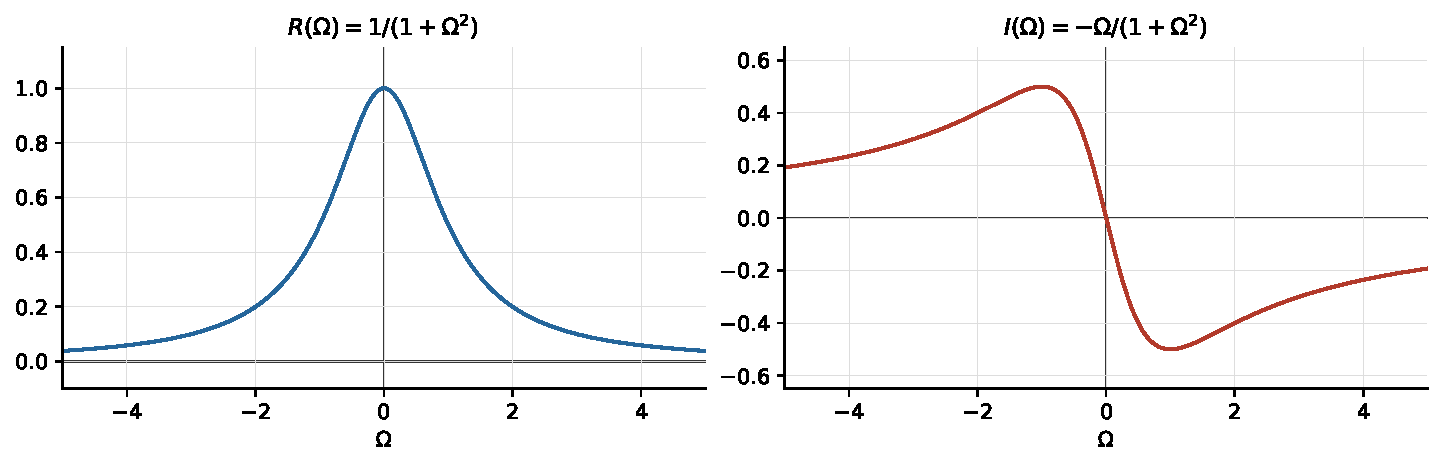
\includegraphics[width=0.92\textwidth]{08-sampling/causal-spectrum-parts.pdf}
  \caption{实因果信号 $\e^{-t}u(t)$ 的频谱实部与虚部。二者满足 $R=\HT_\Omega I$、$I=-\HT_\Omega R$；下标表示沿频率变量作希尔伯特变换。}
  \label{fig:sampling-causal-parts}
\end{figure}

\begin{pitfall}[任意因果广义信号都能照套实虚部关系]
  零时刻的冲激不能当作普通函数的单点删去。\red{零时刻奇异项须另算}。例如 $x(t)=\impulse(t)$ 是因果的，但 $R=1$、$I=0$，由 $I$ 的希尔伯特变换无法得到常数 $1$。使用\cref{eq:sampling-causal-real-imag} 前，应检查衰减、收敛条件及零时刻的奇异项。
\end{pitfall}

\subsection{主值积分与理想移相器}
\label{subsec:sampling-hilbert-definition}

\begin{definition}[希尔伯特变换]
  \keyterm{希尔伯特变换（Hilbert transform）}记为
  \begin{equation}
    \widehat{x}(t)=\HT\{x\}(t)
      =x(t)\conv\pv\frac1{\pi t}
      =\frac1\pi\pv\int_{-\infty}^{\infty}
           \frac{x(\tau)}{t-\tau}\dd\tau.
    \label{eq:sampling-hilbert-definition}
  \end{equation}
  当积分的点态主值存在时，$\pv$ 表示从奇点两侧对称挖去等宽区间：
  \[
    \widehat{x}(t)=\lim_{\varepsilon\to0^+}\frac1\pi
      \left[\int_{-\infty}^{t-\varepsilon}
              \frac{x(\tau)}{t-\tau}\dd\tau
           +\int_{t+\varepsilon}^{\infty}
              \frac{x(\tau)}{t-\tau}\dd\tau\right].
  \]
  \blue{无穷远处也须有适当收敛}。对有限能量信号，可等价地按下面的频域乘子定义，再以均方意义反演。
\end{definition}

\red{奇点两侧对称取主值}，两边的奇异贡献要一起取极限，不能各自当作普通反常积分计算。它的系统关系为
\[
  x(t)\longrightarrow\boxed{\pv\,1/(\pi t)}
       \longrightarrow\widehat{x}(t).
\]
利用第六章由阶跃变换与对偶性质得到的变换对\cref{eq:ctft-hilbert-pair}，
\begin{equation}
  \widehat X(\iu\Omega)=G_{\mathrm H}(\iu\Omega)X(\iu\Omega),
  \qquad
  G_{\mathrm H}(\iu\Omega)=-\iu\operatorname{sgn}(\Omega)
   =\begin{cases}
      -\iu,&\Omega>0,\\
      \iu,&\Omega<0.
    \end{cases}
  \label{eq:sampling-hilbert-response}
\end{equation}
零频取 $G_{\mathrm H}(0)=0$。非零频率幅度均为 $1$；正频率相位为 $-\pi/2$，负频率相位为 $\pi/2$，见\cref{fig:sampling-hilbert-response}。
\red{正负频率反向移相}。两侧移相互为共轭，所以实输入仍给实输出。它不改变非零频率的幅度，也不把每个时域样值都乘以 $-\iu$。

\begin{figure}[H]
  \centering
  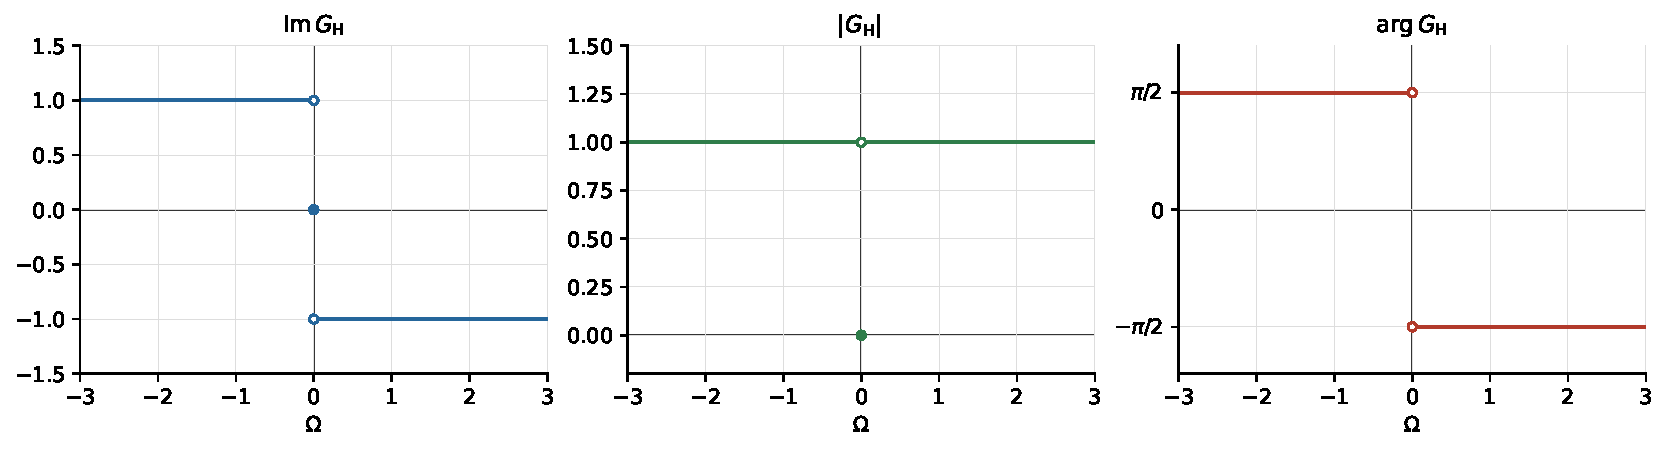
\includegraphics[width=0.94\textwidth]{08-sampling/hilbert-response.pdf}
  \caption{希尔伯特变换器的虚部、幅度和相位。零频乘子取零，因此该点幅度为零、相位未定义；其余频率的幅度为一。}
  \label{fig:sampling-hilbert-response}
\end{figure}

卷积核在负时间也非零，理想变换器是非因果的，也不满足 BIBO 稳定性。例如有界矩形输入 $x(t)=u(t)-u(t-1)$ 的变换为
\[
  \widehat{x}(t)=\frac1\pi\ln\left|\frac{t}{t-1}\right|,
  \qquad t\ne0,1,
\]
在两个端点附近无界。有限能量输入上的均方有界性是另一种性质。实际移相器只能在选定频带内近似实现。

\subsection{反变换、能量与正交性}
\label{subsec:sampling-hilbert-properties}

对有限能量信号，零频的单点不影响反演。非零频率上 $G_{\mathrm H}^2=-1$，两次变换便有
\[
  \HT\{\widehat{x}\}(t)=-x(t).
\]
故希尔伯特反变换为
\begin{equation}
  x(t)=-\HT\{\widehat{x}\}(t)
     =-\frac1\pi\pv\int_{-\infty}^{\infty}
          \frac{\widehat{x}(\tau)}{t-\tau}\dd\tau.
  \label{eq:sampling-inverse-hilbert}
\end{equation}
\red{变换两次得到负号}。\blue{若信号含常数直流项}，按 $G_{\mathrm H}(0)=0$ 的约定该项会被去掉，不能再靠反变换恢复；“两次变换等于负原信号”不能直接套到含直流的周期信号上。

由 $|G_{\mathrm H}|=1$ 几乎处处及帕塞瓦尔关系，
\[
  \int_{-\infty}^{\infty}|\widehat{x}(t)|^2\dd t
    =\frac1{2\pi}\int_{-\infty}^{\infty}|X(\iu\Omega)|^2\dd\Omega
    =\int_{-\infty}^{\infty}|x(t)|^2\dd t.
\]
\red{有限能量保持不变}。对于实有限能量信号，还成立
\begin{equation}
  \int_{-\infty}^{\infty}x(t)\widehat{x}(t)\dd t=0.
  \label{eq:sampling-hilbert-orthogonal}
\end{equation}
证明使用交叉帕塞瓦尔关系：
\begin{align*}
  \int x(t)\widehat{x}(t)\dd t
  &=\frac1{2\pi}\int X(\iu\Omega)\widehat X^*(\iu\Omega)\dd\Omega\\
  &=\frac{\iu}{2\pi}\int
       \operatorname{sgn}(\Omega)|X(\iu\Omega)|^2\dd\Omega=0.
\end{align*}
实信号的 $|X|^2$ 为偶函数，乘上符号函数成为奇函数，故积分为零。\red{实信号与变换正交}。这里的实信号条件不能省去；一般复信号的内积含共轭，也未必为零。正弦等周期信号能量无穷，其正交性应在完整周期上计算。

\subsection{余弦与正弦的变换}
\label{subsec:sampling-hilbert-sinusoid}

设 $\Omega_0>0$。余弦频谱在 $\pm\Omega_0$ 处各有一条权重为 $\pi$ 的冲激。分别乘上两侧的移相增益：
\begin{align*}
  \FT\{\HT[\cos(\Omega_0t)]\}
   &=-\iu\pi\impulse(\Omega-\Omega_0)
       +\iu\pi\impulse(\Omega+\Omega_0)\\
   &=\frac{\pi}{\iu}
       [\impulse(\Omega-\Omega_0)-\impulse(\Omega+\Omega_0)].
\end{align*}
这就是正弦的频谱，所以
\begin{equation}
  \HT[\cos(\Omega_0t)]=\sin(\Omega_0t),
  \qquad
  \HT[\sin(\Omega_0t)]=-\cos(\Omega_0t).
  \label{eq:sampling-hilbert-sinusoid}
\end{equation}
\red{余弦变正弦}，对正频率而言 $\sin(\Omega_0t)=\cos(\Omega_0t-\pi/2)$，恰好是负九十度移相。第二个结果也可\hl{逐条谱线计算}：
\[
  (-\iu)\frac{\pi}{\iu}=-\pi,\qquad
  (\iu)\left(-\frac{\pi}{\iu}\right)=-\pi.
\]
两条权重同为 $-\pi$，反演为 $-\cos(\Omega_0t)$。\red{正弦变负余弦}，不能遗漏负号。\cref{fig:sampling-hilbert-sinusoid} 将两组波形及变换后的谱线对照画出。

\begin{figure}[H]
  \centering
  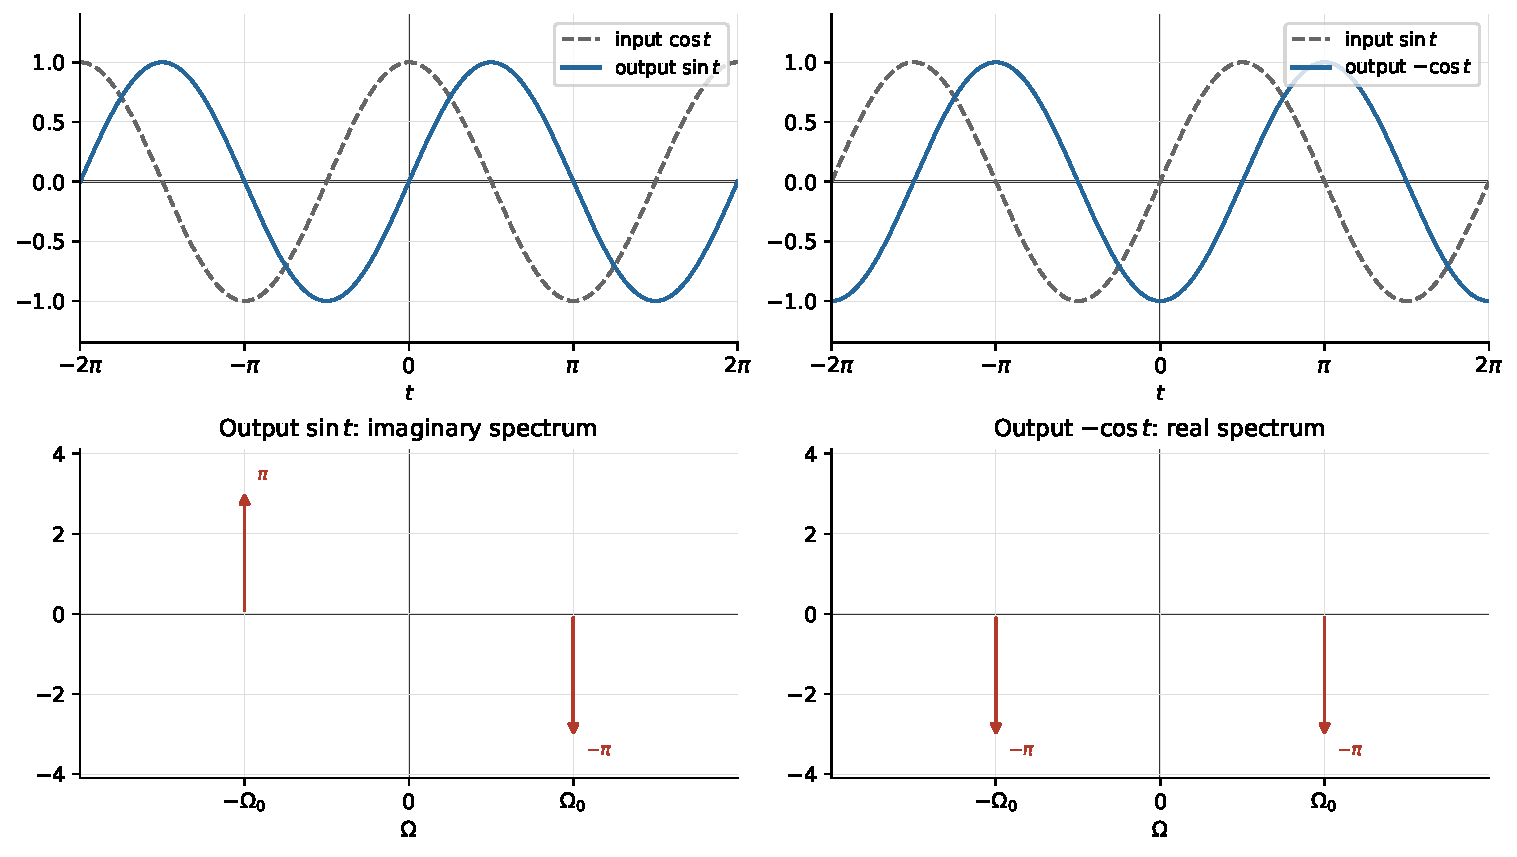
\includegraphics[width=0.94\textwidth]{08-sampling/hilbert-sinusoid.pdf}
  \caption{两组正弦信号的希尔伯特变换，取 $\Omega_0=1$。上行画输入和输出；左下是余弦变换后的虚部谱线，右下是正弦变换后的实部谱线。箭头标权重。}
  \label{fig:sampling-hilbert-sinusoid}
\end{figure}

常相位 $\theta_0$ 可以沿线性性质展开，得到
$\HT[\cos(\Omega_0t+\theta_0)]=\sin(\Omega_0t+\theta_0)$。
若相位或幅度随时间变化，\blue{则需要检查下一节的频带条件}。

\section{窄带信号与瞬时参数}
\label{sec:sampling-instantaneous}

实振荡信号的样值会过零，直接取 $|x(t)|$ \red{得到的是快速起伏}。将 $x$ 与它的希尔伯特变换合成复信号，\red{可以同时描述振荡的幅度和相位}。\blue{以下输入均为实信号}。

\subsection{解析信号与单侧频谱}
\label{subsec:sampling-analytic}

\begin{definition}[解析信号]
  与 $x(t)$ 对应的\keyterm{解析信号（analytic signal）}为
  \begin{equation}
    z(t)=x(t)+\iu\widehat{x}(t).
    \label{eq:sampling-analytic}
  \end{equation}
\end{definition}
由\cref{eq:sampling-hilbert-response}，
\begin{equation}
  Z(\iu\Omega)=[1+\operatorname{sgn}(\Omega)]X(\iu\Omega)
    =\begin{cases}
       2X(\iu\Omega),&\Omega>0,\\
       0,&\Omega<0.
     \end{cases}
  \label{eq:sampling-analytic-spectrum}
\end{equation}
\red{负频率消去}，\red{正频率加倍}。\blue{若有独立的直流谱线}，其权重保持原值。实信号的负频率与正频率共轭，保留一侧即可编码整条实波形；取 $z$ 的实部仍为 $x$。对纯余弦，$z(t)=\cos(\Omega_0t)+\iu\sin(\Omega_0t)=\e^{\iu\Omega_0t}$。

\cref{fig:sampling-analytic-spectrum} 画出窄带实信号的两侧频带与解析信号的单侧频带。它与前面的“因果信号实虚部关系”作用于不同变量：因果性让 $R(\Omega),I(\Omega)$ 构成频率变量上的希尔伯特对；解析信号的 $x(t),\widehat{x}(t)$ 则构成时间变量上的希尔伯特对。解析信号未必因果。

\begin{figure}[H]
  \centering
  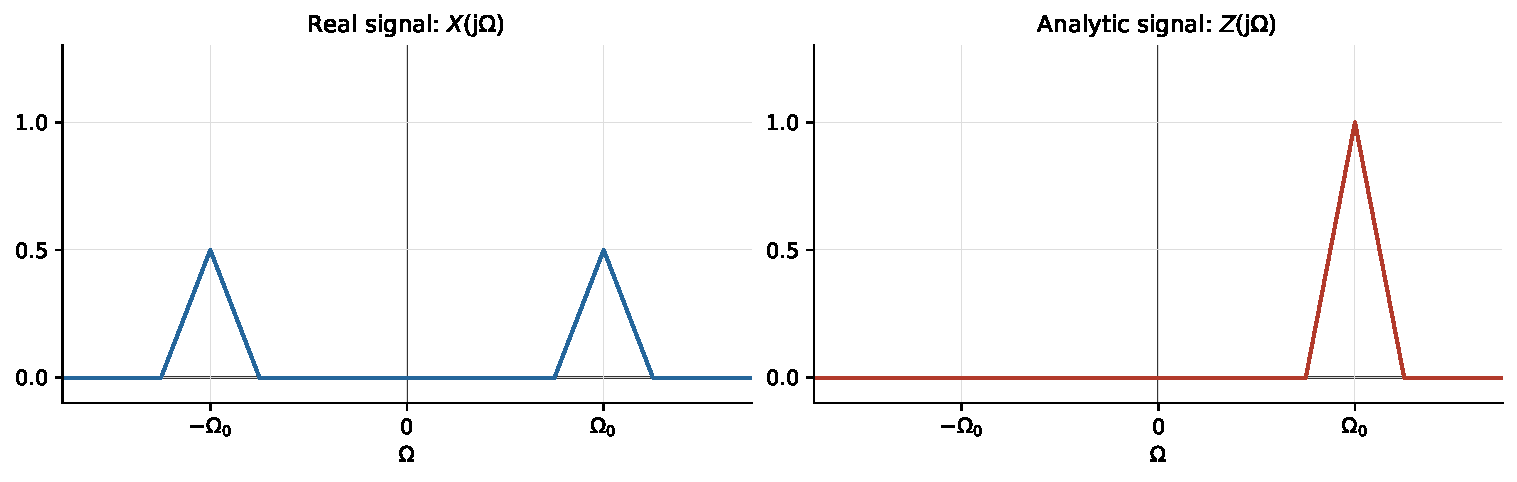
\includegraphics[width=0.92\textwidth]{08-sampling/analytic-spectrum.pdf}
  \caption{窄带实信号与其解析信号的频谱示意。取实偶频谱以便比较高度，正负频带中心为 $\pm\Omega_0$。解析信号只保留正频带，幅度加倍。}
  \label{fig:sampling-analytic-spectrum}
\end{figure}

\subsection{慢变包络与载波的频带条件}
\label{subsec:sampling-narrowband}

\keyterm{窄带信号（narrowband signal）}可写成
\[
  x(t)=a(t)\cos[\Omega_0t+\theta(t)],\qquad \Omega_0>0.
\]
$a(t)$ 描述幅度变化，$\theta(t)$ 描述相对于载波的相位变化。常用近似为
\begin{equation}
  \widehat{x}(t)\approx a(t)\sin[\Omega_0t+\theta(t)],
  \label{eq:sampling-narrowband-approx}
\end{equation}
其前提是 $a,\theta$ 相对于载波变化缓慢，调制后的频带集中在 $\pm\Omega_0$ 附近，且远离零频。\blue{慢变条件先检查}。不能把一般乘积中的 $a(t)$ 随意移出主值积分。

把余弦的和角公式展开：
\[
  x(t)=b(t)\cos(\Omega_0t)-c(t)\sin(\Omega_0t),
  \quad b(t)=a(t)\cos\theta(t),\quad c(t)=a(t)\sin\theta(t).
\]
若 $b,c$ 的频谱均严格支撑在 $|\Omega|\le B<\Omega_0$，则它们与载波的频带分离。此时
\begin{align*}
  \HT[b(t)\cos(\Omega_0t)]&=b(t)\sin(\Omega_0t),\\
  \HT[c(t)\sin(\Omega_0t)]&=-c(t)\cos(\Omega_0t).
\end{align*}
第一式可直接核对：$b\cos$ 的频谱是
$[B_b(\iu(\Omega-\Omega_0))+B_b(\iu(\Omega+\Omega_0))]/2$，
其中 $B_b$ 表示 $b$ 的变换。右侧副本全在正频率，乘 $-\iu$；左侧副本全在负频率，乘 $\iu$。结果恰好是 $b\sin$ 的频谱。第二式同样逐侧相乘即可。

由线性性质，
\begin{align*}
  \widehat{x}(t)
    &=b(t)\sin(\Omega_0t)+c(t)\cos(\Omega_0t)\\
    &=a(t)\sin[\Omega_0t+\theta(t)].
\end{align*}
\red{频带分离时可取等号}。仅知道 $a(t)$ 和 $\theta(t)$ 各自带宽小于 $\Omega_0$，未必能保证 $a\cos\theta$ 和 $a\sin\theta$ 也如此；非线性的 $\cos\theta,\sin\theta$ \red{可能产生更多频率}。一般慢变调制仍按\cref{eq:sampling-narrowband-approx} 的近似处理。常相位、低通包络调幅是容易满足精确条件的情形，见\cref{ex:sampling-envelope}。

\subsection{瞬时包络、相位与频率}
\label{subsec:sampling-instantaneous-parameters}

在 $z(t)\ne0$ 的区间上，把解析信号写成极坐标形式
$z(t)=A(t)\e^{\iu\varphi(t)}$。定义
\begin{equation}
  \begin{aligned}
    A(t)&=|z(t)|=\sqrt{x^2(t)+\widehat{x}^{\,2}(t)},\\
    \varphi(t)&=\arg z(t)\quad\text{（选连续分支）},\\
    \Omega_{\mathrm{inst}}(t)&=\frac{\dd\varphi(t)}{\dd t}.
  \end{aligned}
  \label{eq:sampling-instantaneous-parameters}
\end{equation}
分别称为瞬时包络（instantaneous envelope）、瞬时相位（instantaneous phase）和\keyterm{瞬时角频率（instantaneous angular frequency）}。\blue{相位求导前须选连续分支}；若写成赫兹，则 $f_{\mathrm{inst}}=\Omega_{\mathrm{inst}}/(2\pi)$。

\red{相位要保留象限}。$\arctan(\widehat{x}/x)$ 只给斜率，不能区别第一、第三象限；先用 $\operatorname{atan2}(\widehat{x},x)$ \hl{确定主值相位}，再把相位的 $2\pi$ 跳变展开为连续曲线。\red{求导前展开相位}，否则分支切换会造成虚假的频率尖峰。$A=0$ 处\blue{相位未定义，不能强行求导}；$x=0$ 而 $\widehat{x}\ne0$ 的普通过零点则没有这个问题。

若 $x,\widehat{x}$ 可微且 $A>0$，也可直接计算
\begin{equation}
  \Omega_{\mathrm{inst}}(t)
   =\frac{x(t)\widehat{x}'(t)-\widehat{x}(t)x'(t)}
          {x^2(t)+\widehat{x}^{\,2}(t)}.
  \label{eq:sampling-instantaneous-derivative}
\end{equation}
它来自极角的微分，避免把主值相位跳点直接代入导数。

对满足上一小节精确条件的调制信号，若 $a(t)>0$，有
\[
  z(t)=a(t)\e^{\iu[\Omega_0t+\theta(t)]},\qquad
  A(t)=a(t),\quad
  \varphi(t)=\Omega_0t+\theta(t),\quad
  \Omega_{\mathrm{inst}}(t)=\Omega_0+\theta'(t).
\]
若 $a$ 允许为负，包络应取 $|a|$，负号还会给相位增加 $\pi$；在包络为零处，上述相位和频率关系须另行讨论。\red{包络始终取非负值}。
\cref{fig:sampling-instantaneous-envelope} 对照真实包络、快速振荡及连续相位；一般慢变情况下，与给定 $a,\theta$ 的对应关系也只近似成立。

\begin{figure}[H]
  \centering
  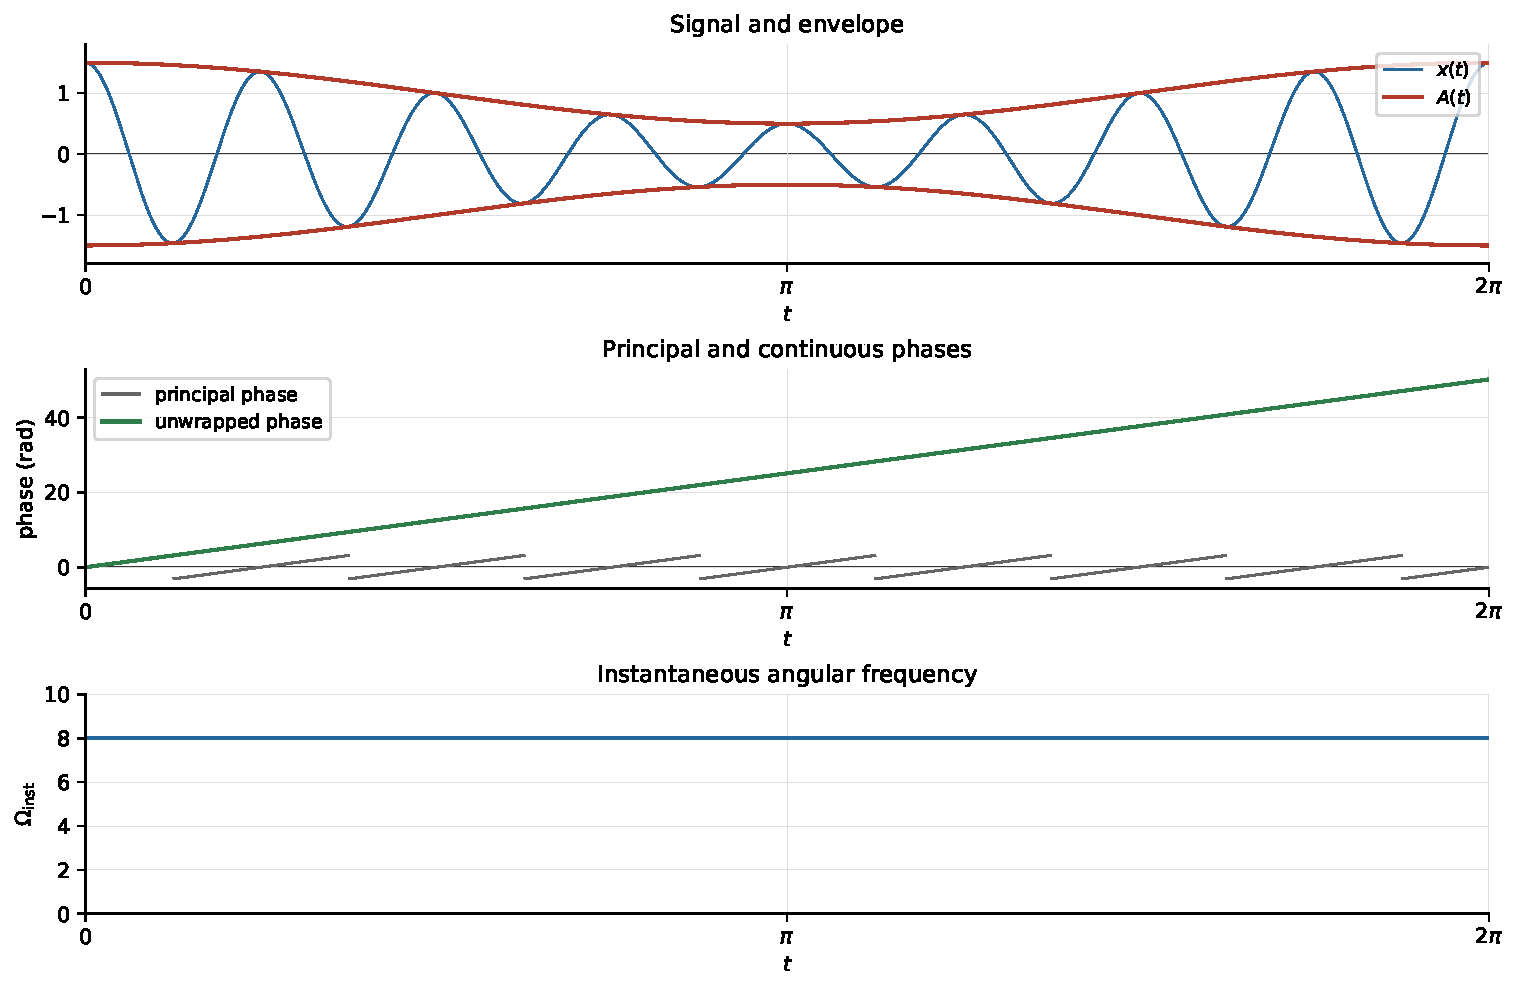
\includegraphics[width=0.94\textwidth]{08-sampling/instantaneous-envelope.pdf}
  \caption{$x(t)=(1+0.5\cos t)\cos(8t)$ 的瞬时参数。上图为信号及上下包络，中图为主值相位与展开相位，下图为瞬时角频率。包络带宽为 $1<8$，因此 $\widehat{x}=(1+0.5\cos t)\sin(8t)$ 精确成立。}
  \label{fig:sampling-instantaneous-envelope}
\end{figure}
\endgroup
